%type de document
\documentclass[12pt,a4paper]{report}

%====================================préambule
%les packages 
%1. traitement des caractères spéciaux
\usepackage[T1]{fontenc}
\usepackage[utf8]{inputenc}
%2. 
 \usepackage[french]{minitoc} 
%\etocsetnexttocdepth{subsection} %list subsections
\usepackage[top=2.5cm, bottom=2.5cm, left=2.5cm, right=2.5cm]{geometry}% geometry package des marges des pages, 
\usepackage[pdftex]{graphicx} %package des images, option pdftex spécifier que le document sera compilé avec pdfLaTeX
\usepackage[colorlinks=false]{hyperref} %for creating links in the pdf version and other additional pdf attributes, no effect on the printed document
\usepackage[final]{pdfpages} %est utilisée pour inclure des pages PDF externes dans votre document LaTeX.final les documents ne sont pas cliquable
\usepackage{float} %pour bien positionner les figures
\usepackage{pslatex} % for times new roman,

\usepackage{array} %  pour créer et personnaliser des tableaux dans votre document
\usepackage{setspace} %pour controler l'espace entre les lignes \onehalfspacing \singlespacing \doublespacing
\usepackage{enumerate}%listes à numéros
\usepackage{longtable}%tableaux sur plusieurs pages
\usepackage{multirow}
\usepackage{placeins} % Dans le préambule
\usepackage{enumitem}%pour des items star fleche etc
\usepackage[french]{babel}
\usepackage[font=small,labelfont=bf]{caption}%les caption seront en taille small et gras(figure1, table1)
\onehalfspacing 

% Définir la longueur de l'espacement entre les paragraphes
\setlength{\parskip}{10pt} % Réglez la valeur selon vos préférences

%pour choisir un style pour les chapitres
%https://latex-tutorial.com/fancy-chapters-latex/
\usepackage[Glenn]{fncychap}
%\usepackage[Conny]{fncychap}
%\usepackage[Bjarne]{fncychap}

% ======Configuration des en-têtes et des pieds de page
\usepackage{fancyhdr}
\pagestyle{fancy}
\fancyhf{}

%\fancyhead[R]{\rightmark} %pour les sections en haut de l'ntête
\fancyhead[LE,RO]{\nouppercase{\leftmark}}  % Chapter name in the outer side of even and odd pages
%lorsque vous utilisez \leftmark dans l'en-tête, LaTeX récupère automatiquement le nom du chapitre en cours. De même, lorsque vous utilisez \rightmark, LaTeX récupère le nom de la section en cours. 
\fancyfoot[LE,RO]{\thepage} % Page number in the outer side of even and odd pages
\fancyfoot[L]{Plateforme de Gestion d'Événements Communautaires }
\renewcommand{\headrulewidth}{0.4pt} % Thickness of the header rule line
\renewcommand{\footrulewidth}{0.4pt} % No footer rule line
%=============document principal ========
\begin{document}

%================insérer toc (sommaire)
\cleardoublepage % Pour commencer une nouvelle page  si nécessaire
\input{projet/Dédicaces.tex}

\chapter*{Remerciements}

%\thispagestyle{empty} % Pour enlever la numérotation de page
Avant de commencer la présentation de ce rapport, nous tenons à exprimer nos  respects et
mes sincères remerciements aux personnels de l'OMINET et nous tenons à remercier le directeur
la société et mon encadreur Yasser BENALI, qui a proposé le sujet de nos projets, et qui a été
Plus qu’un maître de stage. Il  nous a guidés, critiqués et a fait des suggestions.
Son encouragement permanent et son dynamisme organisateur nous ont énormément facilité
La tâche. Il nous a conseillés tout au cours de mon stage. il nous a relu et critiqué mon manuscrit
Nous remercions également toute l’équipe pour son accueil, son esprit convivial et chaleureux.
Enfin, nous tenons à remercier tous ceux qui m’ont assisté à élaborer ce rapport de stage.

\pagenumbering{roman} % Numérotation des pages en chiffres romains
\dominitoc
\tableofcontents
 \listoffigures% liste figures
  \listoftables%liste de tableaux
  \mtcaddchapter 
  %La commande \mtcaddchapter est utilisée avec le package minitoc pour  créer un mini sommaire pour chaque chapitre, affichant les sections et sous-sections qu'il contient.
 \clearpage
 \pagenumbering{arabic}
\chapter*{Introduction Générale}
%ajouter le titre introduction générale dans la table des matières
\addcontentsline{toc}{chapter}{Introduction Générale}
%définir l'entête de ce chapitre 
\markboth{Introduction Générale}{}


Depuis l’émergence de l’informatique, l’homme n’a cessé de développer des langages et des outils pour concevoir le web, mêlant créativité et logique afin de créer des expériences en ligne interactives et fonctionnelles. Aujourd’hui, l’informatique est devenue un pilier central dans la gestion de l’information et un atout majeur dans le monde professionnel en perpétuelle évolution.

Pour les étudiants, acquérir de l’expérience dès leurs études est crucial. Pourtant, la recherche de stages reste un véritable défi : trouver des opportunités alignées avec leurs compétences et aspirations, tout en naviguant dans un écosystème professionnel souvent complexe.

C’est dans cette optique que notre projet prend tout son sens. Nous proposons la création d’une plateforme innovante dédiée à la gestion d’événements. Cet outil offrira aux utilisateurs qu’ils soient simples participants, gestionnaires d’événements ou administrateurs une interface moderne et intuitive pour interagir efficacement.

Les utilisateurs pourront consulter les événements disponibles, s’inscrire, réserver des places en ligne, donner leur avis et échanger avec une communauté dynamique. De leur côté, les administrateurs disposeront d’outils avancés pour organiser et gérer les événements, superviser les inscriptions et analyser les retours des participants, garantissant ainsi une meilleure gestion et une expérience utilisateur optimisée.



\chapter{Présentation du cadre du projet} 
 
 \addcontentsline{toc}{chapter}{Chapitre 1 : Présentation du cadre du projet}
\markboth{Chapitre 1 : Présentation du cadre du projet}{}
\phantomsection % Crée un point d'ancrage pour les hyperliens dans le document
\addcontentsline{toc}{section}{Introduction} % Ajoute "Introduction" dans la table des matières

\section*{Introduction} % Affiche le titre sans numérotation
Dans ce présent chapitre nous avons présenté l’organisme d’accueil, et ses principales activités. Nous avons aussi évoqué la problématique, la solution, l’objectif à atteindre et la planification de notre projet.
\renewcommand{\thesection}{\Roman{section}.} % I, II, ...
\renewcommand{\thesubsection}{\arabic{subsection}.} % 1, 2, ...
\renewcommand{\thesubsubsection}{\thesubsection\arabic{subsubsection}} % I.1, I.2 ...

% Ce qui suit force l’affichage du numéro des subsubsections
\setcounter{secnumdepth}{3} 
\section{Présentation de l'organisme d'accueil}
\subsection{Situation géographique:}
\begin{itemize}
    \item Entreprise : OMINET SARL 
    \item Adresse : Centre Urbain Nord, Tunis. 
    \item Horaires : De 8h à 12h et de 14h à 17h.
\end{itemize}

OMINET SARL, héritière de Coccinet fondée en 2014, est une agence offshore spécialisée dans la création de sites Internet et les solutions digitales sur mesure. Grâce à une équipe d'experts expérimentés, l’entreprise accompagne ses clients dans le développement de leur présence en ligne.

Classée comme une PME (Petite et Moyenne Entreprise), OMINET SARL dispose de plusieurs départements, dont un département commercial et un département technique. L'équipe, composée de [insérer nombre de collaborateurs et stagiaires], est dirigée par un gestionnaire principal.

Depuis sa création, OMINET SARL s'engage à offrir des solutions adaptées aux besoins de ses clients, avec pour objectif principal de maximiser leur satisfaction. L’entreprise met tout en œuvre pour développer des outils digitaux innovants, permettant à ses clients de booster leur performance et d’atteindre leurs objectifs stratégiques.


\subsection{Historique de Coccinet:}
Coccinet est une société à responsabilité limitée (SARL), immatriculée sous le SIREN 479824914, et en activité depuis 18 ans. Basée à Paris (75011), elle se spécialise dans le secteur de la programmation informatique.

Avec un effectif de 6 à 9 salariés, l’entreprise a réalisé un chiffre d'affaires de 200 300 € en 2012, marquant une augmentation notable de 43,64 du total du bilan entre 2011 et 2012.

Depuis sa création, Coccinet a vu plusieurs évolutions importantes, notamment l’enregistrement de différents établissements et mandataires. Le dernier événement notable de l’entreprise remonte au 28 décembre 2021.

Actuellement, l’entreprise est dirigée par Maxence Caillaud, son gérant, qui continue de piloter Coccinet dans ses projets et son développement dans le domaine des solutions informatiques.

\subsection{Organigramme}
L'organigramme de l'OMINET est représenté dans la figure ci-dessous :

\begin{figure}[H]
  \centering
  \begin{minipage}{0.45\textwidth}
    \centering
    
\includegraphics[width=\linewidth]{projet/images/omminet.png}
  \end{minipage}
  \hfill
  \begin{minipage}{0.45\textwidth}
    \centering
    
\includegraphics[width=\linewidth]{projet/images/omminet1.png}
  \end{minipage}
  \caption{L’organigramme de l’OMINET}
\end{figure}
\section{Etude préalable }
\subsection{Critique de l’existant}
En regardant de plus près, voici ce qui pose problème avec ces méthodes :
\begin{itemize}[label=$\rightarrow$]
    \item \textbf{Perte de temps et d’énergie :} \\
    Les organisateurs et participants perdent beaucoup de temps à gérer ou chercher des informations. Et même avec les recherches, les résultats ne sont pas toujours fiables.
    \item \textbf{Problème des places limitées :} \\
    Quand un événement est complet, il n’y a pas de moyen simple pour gérer les gens en liste d’attente. Cela crée de la frustration, car des participants motivés passent à côté.
    \item \textbf{Mauvaise communication :} \\
    Sans système intégré, les annonces ou rappels ne sont pas toujours bien diffusés, ce qui complique la tâche pour tout le monde.
    \item \textbf{Manque d’analyse :} \\
    Il est difficile pour les organisateurs d’avoir une vue claire des statistiques, comme le nombre d’inscrits ou les retours des participants.
    \item \textbf{Plateformes peu adaptées :} \\
    Certaines solutions existantes ne sont pas faites pour de petites structures, soit parce qu’elles sont trop chères, soit parce qu’elles ne correspondent pas aux besoins.
\end{itemize}

\subsection{Problématique:}
Actuellement, les associations, clubs et autres communautés en Tunisie utilisent des méthodes classiques ou des outils simples pour gérer leurs événements, mais ces solutions ne répondent pas toujours à leurs besoins. Voici ce qu’on remarque :
\begin{enumerate}
    \item \textbf{Méthodes traditionnelles :} \\
    Les organisateurs gèrent souvent leurs inscriptions avec des fichiers Excel ou des listes papier. C’est simple mais vite inefficace quand il y a beaucoup de participants.
    \item \textbf{Outils en ligne limités :} \\
    Il existe des plateformes pour créer et gérer des événements, mais elles ne permettent pas forcément de gérer les inscriptions correctement, surtout quand les places sont limitées.
    \item \textbf{Communication dispersée :} \\
    Pour informer les participants, on passe par WhatsApp, des e-mails, ou des publications sur Facebook. C’est compliqué et parfois les gens ratent l’information importante.
    \item \textbf{Peu de retours d’expérience :} \\
    Les outils actuels n’aident pas vraiment à analyser les événements (comme voir combien de personnes se sont inscrites ou ce qui a bien fonctionné).
    \item \textbf{Accessibilité :}  \\
    Certaines plateformes sont trop chères ou compliquées à utiliser pour les petites associations ou clubs.
\end{enumerate}
\subsection{Solution proposée}
Notre plateforme apporte des solutions modernes pour simplifier la gestion des événements et répondre aux besoins des organisateurs :
\begin{itemize}[label=$\star$]
  \item \textbf{Inscriptions faciles :} \\
  Une interface intuitive permet de gérer les inscriptions, les annulations, et les listes d’attente automatiquement.
  \item \textbf{Communication rapide :} \\
  Avec un système de messagerie intégré et des notifications push, les organisateurs peuvent rester connectés avec les participants en temps réel.
  \item \textbf{Suivi clair :} \\
  Un tableau de bord analytique fournit des statistiques sur les inscriptions et les retours des participants, aidant les organisateurs à mieux planifier.
  \item \textbf{Accessibilité pour tous :} \\
  Simple, abordable et adaptée même aux petites communautés, la plateforme est facile à prendre en main sans expertise technique.
  \item \textbf{Gestion des places limitées :} \\
  Les participants peuvent rejoindre une liste d’attente et être notifiés dès qu’une place est disponible.
\end{itemize}
\section {Méthodologie adaptées}
Dans cette section, nous examinons en détail les méthodes utilisées qui nous ont permis de progresser dans la réalisation de notre projet.
\subsection{Méthodologie de modélisation et de conception}
En utilise le méthodologie de modélisation et de conception  pour mieux comprendre les besoins et planifier techniquement le projet .

Le langage UML (Unified Modeling Language, ou langage de modélisation unifié) a été pensé pour être un langage de modélisation visuelle commun, et riche sémantiquement et syntaxiquement.Son objectif est de concevoir et mettre en place des systèmes logiciels complexes en termes de structure et de comportement. Les applications de l’UML dépassent le domaine du développement logiciel, en particulier pour les flux de processus dans le secteur industriel.\cite{ref1}
\subsection{Methodologie de gestion de projet }
Dans le domaine de developpement web , les projets informatiques deviennent de plus en plus complexes avec l’évolution rapide des technologies et des besoins , alors en va Développer une approche stratégique pour repondre au besoin du client car les anciennes méthodes de gestion rigides ne répondent plus à cette réalité . dans ce cas l’approche Agile s’est imposée comme une solution moderne et efficace.

La méthode agile est une méthode de gestion de projet. L’idée, lorsque l’on utilise cette approche, est d’apporter souplesse et performance à la gestion de projet. Centrée sur l’humain et la communication, elle permet aux clients de participer au développement d’un produit tout au long de l’avancement du projet.\cite{ref2} .
Dans ce maniére en utilise le méthode SCRUM pour ce projet 

Scrum C'est la méthode de travail la plus répandue pour la gestion des projets agile et divise le travail dans un équipe .

Scrum est une structure Agile qui facilite la collaboration au sein des équipes et les aide à réaliser des tâches à haute valeur ajoutée. Elle propose un schéma de valeurs, rôles et directives pour leur permettre de se concentrer sur chaque itération et de s’améliorer en continu.\cite{ref3}

\textbf{Principes fondamentaux : }\\
\textbf{•	Collaboration :   } Les équipes travaillent ensemble de manière collaborative. \\
\textbf{•	Itération } Le travail est divisé en sprints (généralement de 2 à 4 semaines). \\
\textbf{•	Adaptabilité }Les exigences peuvent évoluer en fonction des retours des utilisateurs.
\subsubsection{Rôles dans Scrum :}
Le methode scrum définit trois rôles principaux :

 \begin{itemize}
    \item[$\star$] \textbf{Product Owner : }traduit les besoins du client en tâches concrètes pour l’équipe, tout en s’assurant que les priorités sont claires et alignées avec les objectifs du projet. 
 \item[$\star$]\textbf{Scrum Master : }il accompagne l’équipe au quotidien en veillant à ce que le cadre Scrum soit respecté, tout en aidant chacun à avancer malgré les blocages éventuels.
 \item[$\star$]\textbf{Équipe de Développement : } qui transforme les idées en solutions concrètes, en collaborant activement pour livrer un produit fonctionnel et de qualité . 
\end{itemize}
\subsubsection{ Artefacts de Scrum :}
Les artefacts de scrum permet de  de gérer le travail .
 \begin{itemize}
\item[$\star$] \textbf{Product Backlog : } Il contient toutes les idées, fonctionnalités et améliorations à venir. Il se met à jour au fur et à mesure que le projet avance, afin de s’assurer que les priorités restent alignées avec les besoins réels du client.
\item[$\star$]\textbf{Sprint Backlog : } C’est la liste des tâches que l’équipe doit accomplir en fonction de ses capacités et des priorités du moment, choisies directement à partir du Product Backlog
\item[$\star$]\textbf{ Increment : }C'est un livrable qui doit être fonctionnel et prêt à être déployé, garantissant que chaque itération apporte une réelle valeur ajoutée au projet.
\end{itemize}
\subsubsection{Processus Scrum : }
Le Processus Scrum comporte plusieurs étapes.
 \begin{itemize}
    \item[$\star$] \textbf{ sprint meeting planning : } Est un moment où l'équipe trier les éléments du product backlog à réaliser durant le sprint.
et définies les tâches spécifiques  pour chaque élément sélectionné.
      \item[$\star$] \textbf{ Daily Scrum : }  faire une réunion quotidienne de 15 minutes pour cadrer l'équipe et chaque membre partage son travail et  présente les difficultés rencontrées.
       \item[$\star$] \textbf{Le sprint review : } le Product Owner invite l’équipe Scrum et les parties prenantes, et l’équipe presente ce qu’il  a fait.Les parties prenantes donnent leur avis, pour permet d'améliorer le produit et d’ajuster le backlog.
        \item[$\star$] \textbf{Sprint Rétrospective : } c'est la dernier réunions ,on discute sur ce qui a bien fonctionné et ce qui peut être amélioré .
\end{itemize}
\begin{figure}[H]
    \centering
    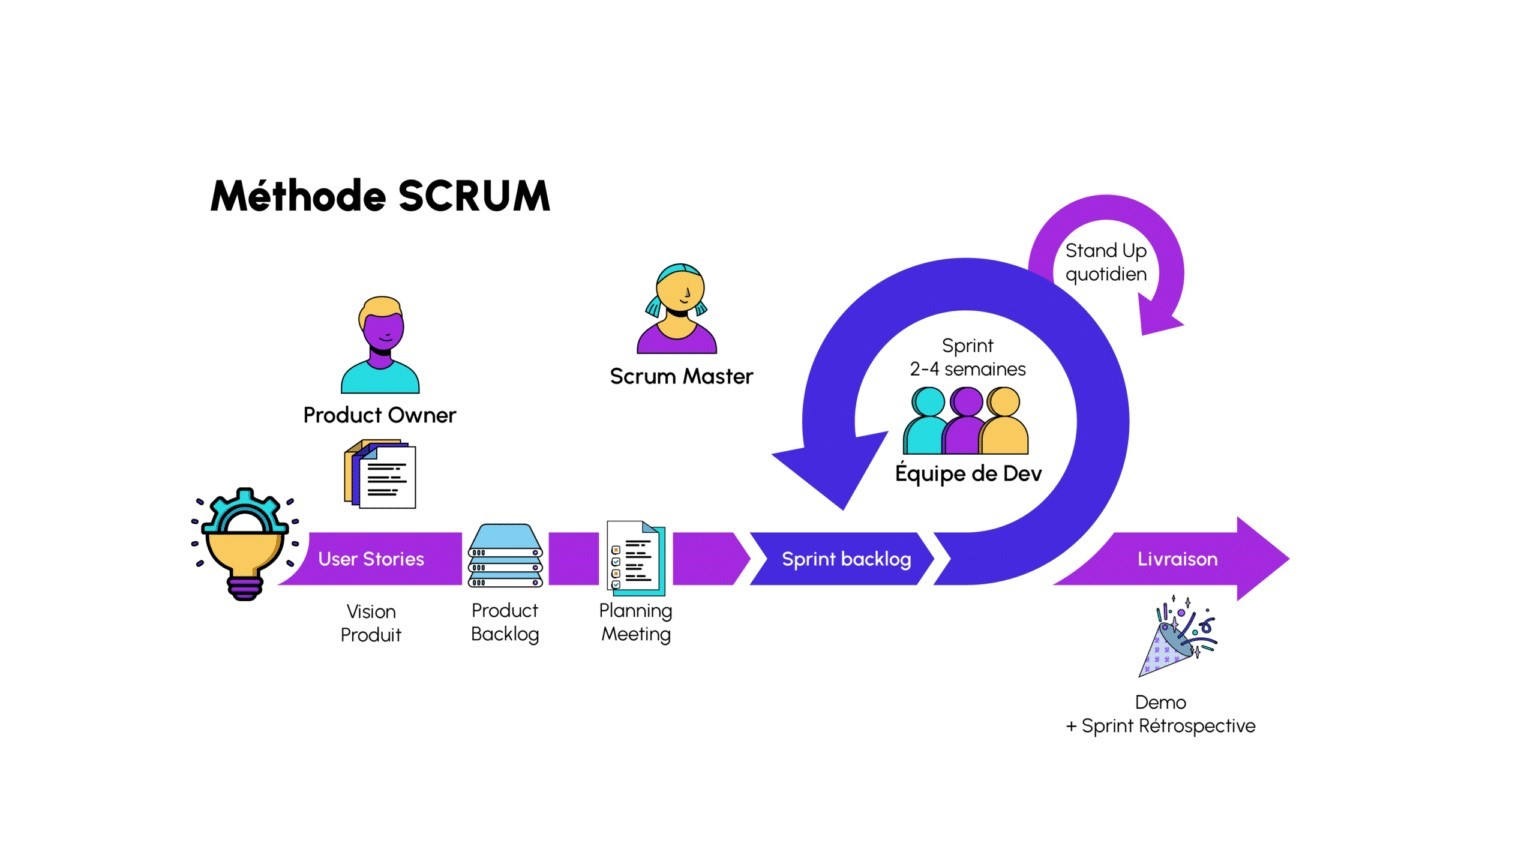
\includegraphics[width=0.9\linewidth]{projet/images/methodeScrum.jpg}
    \caption{ Le processus de Scrum}
    \label{fig:image_centree}
\end{figure}


\addcontentsline{toc}{section}{Conclusion}
\section*{Conclusion}
Au cours de ce chapitre, nous avons présenté la société d’accueil « OMINET » ainsi que l’étude préalable, les méthodologies utilisées.
Dans le prochain chapitre, notre objectif est la planification du projet

\chapter{Planification du projet}
\addcontentsline{toc}{chapter}{Chapitre 2 : Planification du projet}

 

 \addcontentsline{toc}{section}{Introduction} % Ajoute "Introduction" dans la table des matières

\section*{Introduction}
Dans ce chapitre, nous allons en premier lieu définir les acteurs en détaillant les besoins fonctionnels et non fonctionnels de notre application. En second lieu, nous allons présenter l’architecture de notre plateforme.
% Numérotation

\renewcommand{\thesection}{\Roman{section}.} 
\renewcommand{\thesubsection}{\arabic{subsection}.}
\renewcommand{\thesubsubsection}{\thesubsection\arabic{subsubsection}}
% Section 1

\section{Spécification des besoins}


\subsection{Besoins fonctionnels}
Notre application permet à Administrateur :
\begin{itemize}
    \item Gérer les utilisateurs.
    \item Gérer les événements.
    \item Gérer les catégories.
    \item Consulter les statistiques.
\end{itemize}

Notre application permet à Gestionnaire des événements :
\begin{itemize}
    \item Créer un compte.
    \item Mettre à jour son profil.
    \item Gérer les événements.
    \item Gérer les inscriptions.
    \item Envoyer des rappels.
    \item Accéder aux statistiques des événements.
\end{itemize}

Notre application permet à Utilisateur :
\begin{itemize}
    \item Créer un compte.
    \item Mettre à jour son profil.
    \item Lister les événements.
    \item S’inscrire à un événement.
    \item Envoyer des messages pour demande d'information.
    \item Faire un commentaire.
\end{itemize}

\subsection{Besoins non fonctionnels}

\subsubsection*{Performance:}
\begin{itemize}
    \item La plateforme doit supporter jusqu’à 500 utilisateurs simultanés sans dégrader les performances.
\end{itemize}

\subsubsection*{Sécurité:}
\begin{itemize}
    \item Les mots de passe doivent être cryptés pour garantir leur sécurité.
    \item Des règles strictes d’accès aux données doivent être définies selon les rôles.
    \item La plateforme doit être protégée contre les attaques comme les injections SQL et XSS.
\end{itemize}

\subsubsection*{Fiabilité:}
\begin{itemize}
    \item La plateforme doit être disponible 99,9\% du temps avec un minimum de temps d’arrêt.
    \item Les données doivent être sauvegardées quotidiennement pour éviter leur perte.
\end{itemize}

\subsubsection*{Scalabilité:}
\begin{itemize}
    \item L’architecture doit évoluer pour supporter une augmentation d’utilisateurs et d’événements.
    \item Il doit être facile d'ajouter de nouvelles fonctionnalités à la plateforme.
\end{itemize}

\subsubsection*{Accessibilité:}
\begin{itemize}
    \item La plateforme doit respecter les normes d’accessibilité (WCAG 2.1).
    \item Elle doit être compatible avec les lecteurs d’écran et utiliser des couleurs contrastées.
\end{itemize}

\subsubsection*{Maintenabilité:}
\begin{itemize}
    \item Le code doit être bien structuré, documenté et facile à modifier.
    \item Des tests automatisés doivent être utilisés pour détecter rapidement les erreurs.
\end{itemize}

\subsubsection*{Portabilité:}
\begin{itemize}
    \item La plateforme doit être compatible avec les navigateurs principaux (Chrome, Firefox, Edge, Safari).
    \item L’hébergement doit se faire sur des serveurs cloud (AWS, Azure).
\end{itemize}

% Section 2
\section{Gestion de projet avec Scrum}

\subsection{Équipe SCRUM et rôles}
SCRUM définit trois rôles, comme reflété dans la figure ci-dessous :\\
— Product Owner : Mr. Yasser Ben Ali\\
— Scrum Master : Mme. Hella Jebali\\
— L’équipe de développement : Wided Laabidi et Mohamed Aziz Barrouta

\begin{figure}[H]
    \centering
    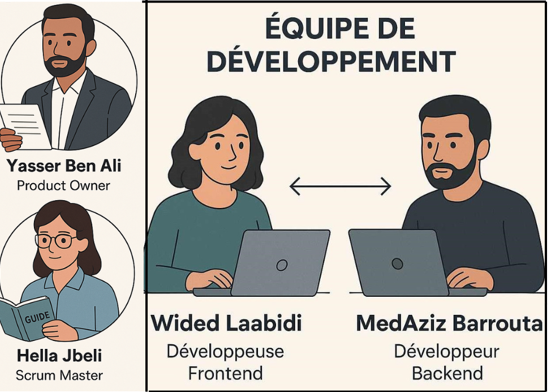
\includegraphics[width=0.7\linewidth]{projet/images/equipeScrum.png}
    \caption{L'équipe Scrum}
    \label{fig:equipe_scrum}
\end{figure}

\subsection{Product Backlog}
C'est le composant le plus basique dans le processus Scrum. Nous l’avons utilisé pour
Planifier la réalisation de chaque sprint. Donc, il contient des fonctionnalités
requises pour la construction d’un produit, ainsi que tous les éléments nécessitant
L’intervention de l’équipe. Ces éléments sont classés par ordre de priorité et de
Leur dépendance, ce qui permet de spécifier l’ordre de leur réalisation.\\


\begin{table}[h!]
\renewcommand{\arraystretch}{1.6}
\setlength{\tabcolsep}{5pt}
\centering
\begin{tabular}{|c|c|m{7cm}|c|c|}
\hline
\textbf{ID} & \textbf{Sprint} & \textbf{User Story} & \textbf{Priorité} & \textbf{Complexité} \\
\hline


\multirow{3}{*}{2} & \multirow{3}{*}{\parbox{3cm}{\centering Authentification\\ et gestion des utilisateurs}} 
& En tant qu’utilisateur , je veux m’inscrire et me connecter pour accéder à mon espace.. & Élevé & Moyenne \\
\cline{3-5}
&& En tant que gestionnaire , je veux m’inscrire et me connecter pour accéder à mon espace.. & Élevé & Moyenne \\
\cline{3-5}
& & En tant qu’administrateur, je veux gérer les rôles des utilisateurs pour contrôler l’accès.. & Élevé & Moyenne \\
\cline{3-5}
\hline


\multirow{7}{*}{3} & \multirow{7}{*}{\parbox{3cm}{\centering Gestion\\ des évenements }} 
& En tant qu’administrateur, je veux  modifier  des événements. & Élevé & Moyenne \\
\cline{3-5}
& & En tant qu’administrateur, je veux supprimer des événements. & Élevé & Moyenne \\
\cline{3-5}
& & En tant qu’administrateur, je veux Consulter des événements. & Élevé & Moyenne \\
\cline{3-5}
& & En tant qu’administrateur, je veux Approver des événements. & Élevé & Moyenne \\
\cline{3-5}
& & En tant que Gestionnaire , je veux Créer des événements. & Élevé & Moyenne \\
\cline{3-5}
& & En tant que Gestionnaire, je veux Modifier des événements. & Élevé & Moyenne \\
\cline{3-5}
& & En tant que Gestionnaire, je veux Supprimer  des événements. & Élevé & Moyenne \\
\hline

\multirow{3}{*}{4} & \multirow{3}{*}{\parbox{3cm}{\centering  Inscription et\\  interaction utilisateur }} 
& qu’utilisateur, je veux m’inscrire à un événement. & Élevé & Moyenne \\
\cline{3-5}
& & En tant qu’utilisateur, je veux recevoir une notification après inscription. & Élevé & Moyenne \\
\cline{3-5}
& & En tant qu’utilisateur, je veux laisser un feedback après participation. & Élevé & Moyenne \\

\hline
\multirow{3}{*}{5} & \multirow{3}{*}{\parbox{3cm}{\centering Gestion avancée \\et tableaux de bord }} 
& En tant qu’utilisateur, je consulte les statistique globales & Haute  & Moyenne \\
\cline{3-5}
& & En tant que Geestionnaire j'accéder au statistique des évenement  & Élevé & Moyenne \\
\cline{3-5}
\hline
\end{tabular}
\caption{Product Backlog}
\end{table}

\clearpage
\subsection{Planification de sprint}
La préparation des sprints revêt une importance capitale dans la concrétisation des projets
SCRUM. Nous diviserons notre projet en 4 releases qui seront constituées de 6 sprints. La figure
suivante illustre la division des releases en sprints.
\begin{figure}[H]
    \centering
    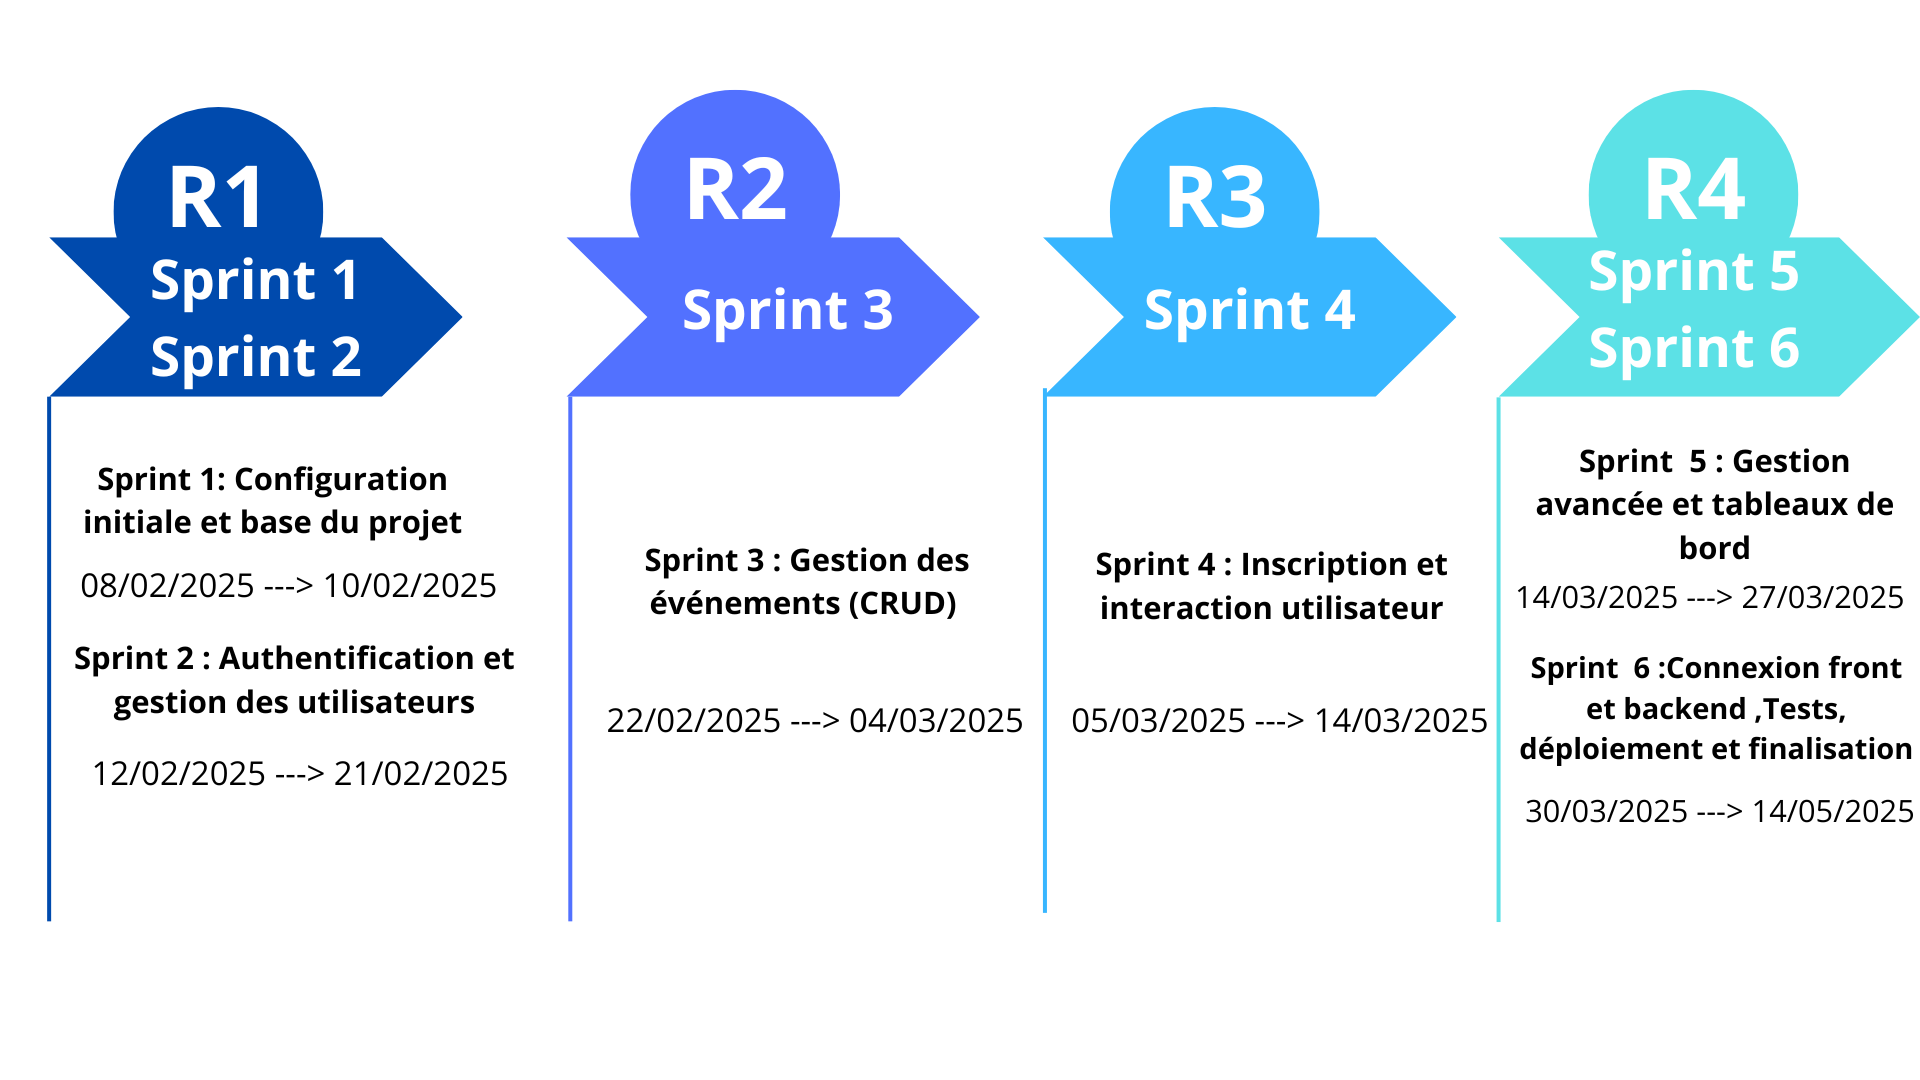
\includegraphics[width=0.9\linewidth]{projet/images/R1.png}
    \caption{Planification des sprints}
    \label{fig:equipe_scrum}
 \end{figure}

% Section 3
\section{Diagrammes de cas d'utilisations général}

\subsection{Identification des acteurs}

Dans cette section, nous définissons les acteurs du système ainsi que leurs rôles respectifs. Le tableau~\ref{tab:identification_acteurs} ci-dessous récapitule ces informations.

\begin{longtable}{|p{4cm}|p{5cm}|p{6cm}|}
\hline
\textbf{Acteur} & \textbf{Rôle} & \textbf{Fonctionnalités/Services} \\ 
\hline
\parbox[c][3.5cm][c]{\linewidth}{\centering

\includegraphics[width=0.3\linewidth]{projet/images/acteur.jpg} \\[0.2cm] \textbf{Administrateur}
} & 
Gérer et administrer la plateforme & 
\begin{itemize}[leftmargin=0.5cm]
    \item Gérer les utilisateurs.
    \item Gérer les événements.
    \item Consulter les statistiques.
\end{itemize} \\ 
\hline

\parbox[c][3.5cm][c]{\linewidth}{\centering

\includegraphics[width=0.3\linewidth]{projet/images/acteur.jpg} \\[0.2cm] \textbf{Utilisateur}
} & 
Participer aux événements & 
\begin{itemize}[leftmargin=0.5cm]
    \item S’inscrire aux événements.
    \item Envoyer des messages.
    \item Poster des commentaires.
\end{itemize} \\ 
\hline

\parbox[c][3.5cm][c]{\linewidth}{\centering

\includegraphics[width=0.3\linewidth]{projet/images/acteur.jpg} \\[0.2cm] \textbf{Gestionnaire des événements}
} & 
Organiser et gérer les événements & 
\begin{itemize}[leftmargin=0.5cm]
    \item Créer et modifier des événements.
    \item Gérer les inscriptions.
    \item Suivre les statistiques des événements.
\end{itemize} \\ 
\hline
\caption{Identification des acteurs et de leurs fonctionnalités}
\label{tab:identification_acteurs}
\end{longtable}

% Section 4

\subsection{Diagramme de contexte statique}
Ce diagramme UML montre la relation des différents acteurs avec le système.

\begin{figure}[H]
    \centering
    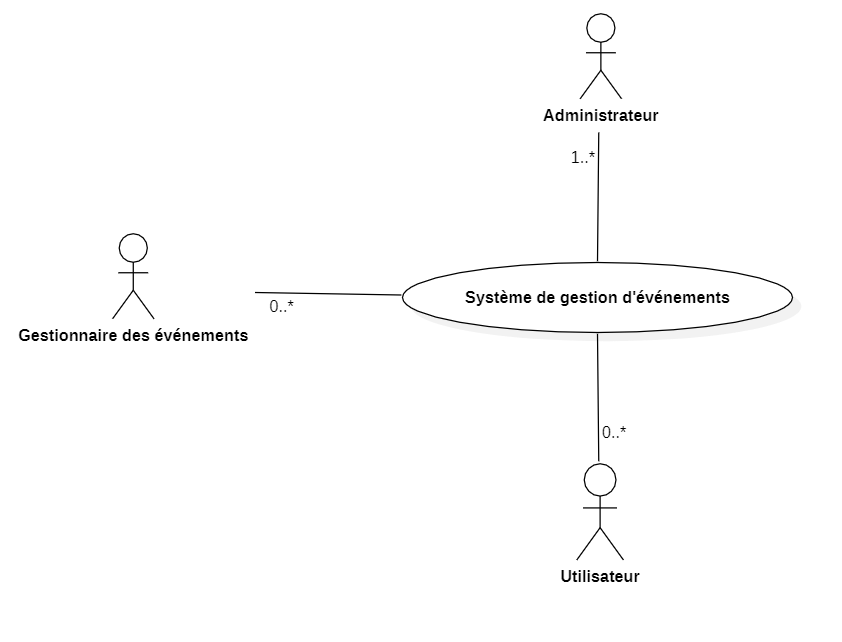
\includegraphics[scale=0.3]{projet/images/Diagramme de contexte statique.png}
    \caption{Diagramme de contexte statique}
\end{figure}

% Section 5
\subsection{Diagramme de cas d’utilisation global}
Voici le diagramme de cas d’utilisation global de notre application :

\begin{figure}[H]
    \centering
    \includegraphics[width=\textwidth]{projet/images/Diagramme de cas d’utilisation global.png}
    \caption{Diagramme de cas d'utilisation globale}
\end{figure}

\section{Diagramme de classes général}

Ce diagramme UML représente la structure de données de notre application.

\begin{figure}[H]
    \centering
    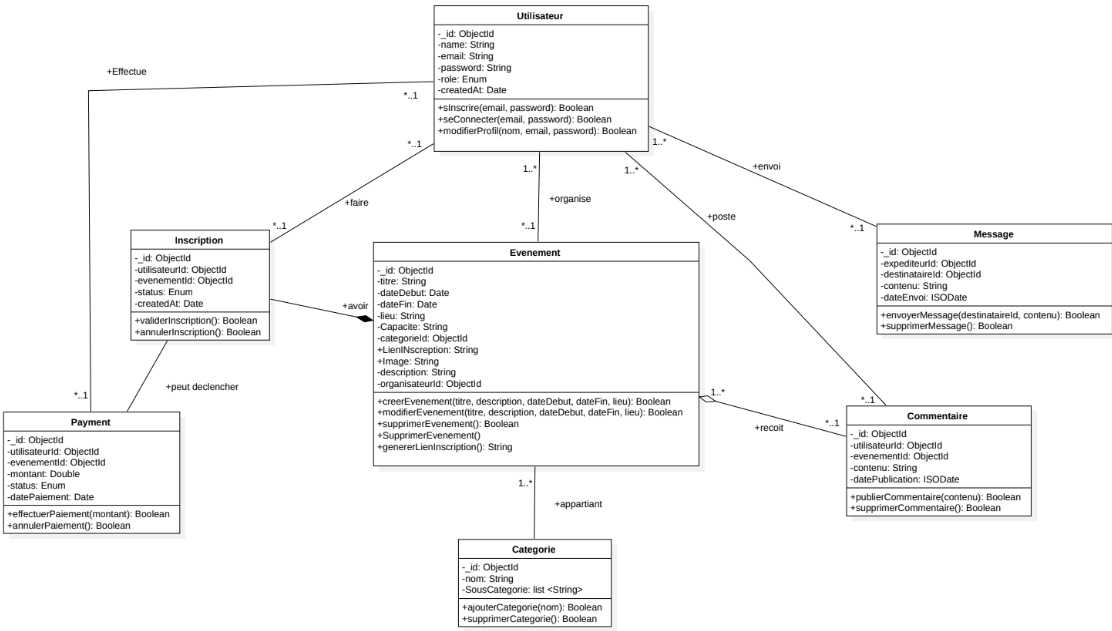
\includegraphics[width=0.95\textwidth]{projet/images/diagramme de classe.png}
    \caption{Diagramme de classes général de l'application}
    \label{fig:diagramme_classe}
\end{figure}

\section{Environnement de développement et choix techniques}

Dans cette section, nous présentons l’environnement matériel ainsi que l’environnement logiciel utilisés pour implémenter la solution informatique.

\subsection{Environnement matériel}

Nous détaillons ici les caractéristiques matérielles, notamment le processeur, la mémoire vive (RAM), le disque dur et le système d’exploitation de chaque ordinateur utilisé. Toutes les informations sont récapitulées dans le Tableau ~\ref{tab:environnement_materiel}.

\begin{table}[H]
\centering
\begin{tabular}{|l|l|l|}
\hline
\textbf{Ordinateur} & \textbf{1} & \textbf{2} \\ \hline
Propriétaire & Laabidi Wided & Barrouta Mouhamed Aziz \\ \hline
Processeur & Intel Core i5 & AMD Ryzen 5 \\ \hline
RAM & 16 Go & 8 Go \\ \hline
Disque Dur & 476 Go SSD & 512 Go SSD \\ \hline
Système d’exploitation & Windows 10 (64 bits) & Windows 11 (64 bits) \\ \hline
\end{tabular}
\caption{Caractéristiques matérielles des ordinateurs utilisés}
\label{tab:environnement_materiel}
\end{table}
\subsection{Environnement logiciel}
Dans cette sous-section, nous décrivons les différents logiciels informatiques
que nous avons utilisé pour mener à terme notre projet.
\begin{figure}[H]
    \centering
    \begin{minipage}[c]{0.3\textwidth}
      
\includegraphics[width=\linewidth]{projet/images/vs code.png}
    \end{minipage}
    \hspace{1cm}
    \begin{minipage}[c]{0.6\textwidth}
        \textbf{Visual Studio Code (VS Code).}\\[0.5em]
        Est un éditeur de code source et un environnement de développement intégré (IDE) de Microsoft. Il est open-source et cross-platform, c’est-à-dire qu’il fonctionne sur Windows, Linux et Mac. Il a été conçu pour les développeurs web, mais il prend en charge de nombreux autres langages de programmation tels que C++, C#, Python, Java, etc.
    \end{minipage}
\end{figure}

\vspace{0.5cm}

\begin{figure}[H]
    \centering
    \begin{minipage}[c]{0.3\textwidth}
        
\includegraphics[width=\linewidth]{projet/images/PostMan.png}
    \end{minipage}
    \hspace{1cm}
    \begin{minipage}[c]{0.6\textwidth}
        \textbf{Postman.}\\[0.5em]
        Est une plateforme API tout-en-un pour la création et l'utilisation d'API. Elle simplifie chaque étape du cycle de vie des API : de la conception et des tests à la livraison et à la surveillance. \cite{ref5}
    \end{minipage}
\end{figure}

\vspace{0.5cm}

\begin{figure}[H]
    \centering
    \begin{minipage}[c]{0.3\textwidth}
        
\includegraphics[width=\linewidth]{projet/images/Node JS.png}
    \end{minipage}
    \hspace{1cm}
    \begin{minipage}[c]{0.6\textwidth}
        \textbf{Node Js.}\\[0.5em]
        Est un environnement d'exécution JavaScript gratuit, open source et multiplateforme qui permet aux développeurs de créer des serveurs, des applications Web, des outils de ligne de commande et des scripts. \cite{ref6}
    \end{minipage}
\end{figure}

\vspace{0.5cm}

\begin{figure}[H]
    \centering
    \begin{minipage}[c]{0.3\textwidth}
        
\includegraphics[width=\linewidth]{projet/images/GITHUB.png}
    \end{minipage}
    \hspace{1cm}
    \begin{minipage}[c]{0.6\textwidth}
        \textbf{GitHub.}\\[0.5em]
        Est une plateforme open source de gestion de versions et de collaboration destinée aux développeurs de logiciels. \cite{ref7}
    \end{minipage}
\end{figure}

\vspace{0.5cm}

\begin{figure}[H]
    \centering
    \begin{minipage}[c]{0.3\textwidth}
        
\includegraphics[width=\linewidth]{projet/images/Overleaf.png}
    \end{minipage}
    \hspace{1cm}
    \begin{minipage}[c]{0.6\textwidth}
        \textbf{Overleaf.}\\[0.5em]
        Est un éditeur LaTeX en ligne et collaboratif. Il inclut un environnement LaTeX complet, prêt à l’emploi et permet de produire des documents scientifiques de haute qualité. \cite{ref8}
    \end{minipage}
\end{figure}
\vspace{0.5cm}

\begin{figure}[H]
    \centering
    \begin{minipage}[c]{0.3\textwidth}
        
\includegraphics[width=\linewidth]{projet/images/téléchargement.jpg}
    \end{minipage}
    \hspace{1cm}
    \begin{minipage}[c]{0.6\textwidth}
        \textbf{Canva.}\\[0.5em]
        Lancé en 2013, Canva est un outil de design et de communication visuelle en ligne dont la mission est de permettre à tout le monde de concevoir et de publier selon ses envies.\cite{ref27}
    \end{minipage}
\end{figure}

\
\subsection{Les langages de programmation}
\begin{figure}[H]
    \centering
    \begin{minipage}[c]{0.3\textwidth}
      
\includegraphics[width=\linewidth]{projet/images/HTML5.png}
    \end{minipage}
    \hspace{1cm}
    \begin{minipage}[c]{0.6\textwidth}
        \textbf{HTML5.}\\[0.5em]
        Signifie « HyperText Markup Language » qu'on peut traduire par « langage de balises pour l'hypertexte ». Il est utilisé afin de créer et de représenter le contenu d'une page web et sa structure\cite{ref9}
    \end{minipage}
\end{figure}

\vspace{0.5cm}

\begin{figure}[H]
    \centering
    \begin{minipage}[c]{0.3\textwidth}
        
\includegraphics[width=\linewidth]{projet/images/CSS3.png}
    \end{minipage}
    \hspace{1cm}
    \begin{minipage}[c]{0.6\textwidth}
        \textbf{CSS.}\\[0.5em]
      Le CSS pour Cascading Style Sheets est un langage informatique uti-
lisé sur Internet pour la mise enforme de fichiers et de pages HTML.\cite{ref10}
    \end{minipage}
\end{figure}

\vspace{0.5cm}

\begin{figure}[H]
    \centering
    \begin{minipage}[c]{0.3\textwidth}
        
\includegraphics[width=\linewidth]{projet/images/JavaScript.png}
    \end{minipage}
    \hspace{1cm}
    \begin{minipage}[c]{0.6\textwidth}
        \textbf{JavaScript.}\\[0.5em]
       Est un langage de script qui vous permet de créer du contenu
mis à jour dynamiquement, de contrôler le multimédia, d’animer des
images. \cite{ref11}
    \end{minipage}
\end{figure}

\vspace{0.5cm}

\begin{figure}[H]
    \centering
    \begin{minipage}[c]{0.3\textwidth}
        
\includegraphics[width=\linewidth]{projet/images/latex.png}
    \end{minipage}
    \hspace{1cm}
    \begin{minipage}[c]{0.6\textwidth}
        \textbf{LaTeX.}\\[0.5em]
        Est un système logiciel de composition de documents créé par Leslie Lamport. Plus exactement, il s'agit d'une collection de macro-commandes destinées à faciliter l'utilisation du « processeur de texte » TeX de Donald Knuth. Il a été créé en 1985. \cite{ref12}
    \end{minipage}
\end{figure}
\subsection{Framework}
\begin{figure}[H]
    \centering
    \begin{minipage}[c]{0.3\textwidth}
        
\includegraphics[width=\linewidth]{projet/images/Tailwind-CSS.png}
    \end{minipage}
    \hspace{1cm}
    \begin{minipage}[c]{0.6\textwidth}
        \textbf{Tailwind-CSS.}\\[0.5em]
        Est est un framework CSS open source. La fonctionnalité principale de cette bibliothèque est, contrairement à d'autres frameworks CSS comme Bootstrap, qu'elle ne procure pas une série de classes prédéfinies pour des éléments tels que des boutons ou des tables.\cite{ref13}
    \end{minipage}
\end{figure}
\vspace{0.5cm}

\begin{figure}[H]
    \centering
    \begin{minipage}[c]{0.3\textwidth}
        
\includegraphics[width=\linewidth]{projet/images/express.png}
    \end{minipage}
    \hspace{1cm}
    \begin{minipage}[c]{0.6\textwidth}
        \textbf{Express.Js.}\\[0.5em]
     Est le framework backend le plus populaire pour Node.js, et il fait partie intégrante de l’écosystème JavaScript.Il est conçu pour construire des applications web monopages, multipages et hybrides, il est également devenu la norme pour le développement d’applications backend avec Node.js, et il constitue la partie backend de ce que l’on appelle la pile MEVN. \cite{ref14}
    \end{minipage}
\end{figure}
\subsection{Le système de gestion de base de données}
\begin{figure}[H]
    \centering
    \begin{minipage}[c]{0.3\textwidth}
        
\includegraphics[width=\linewidth]{projet/images/mongodb.png}
    \end{minipage}
    \hspace{1cm}
    \begin{minipage}[c]{0.6\textwidth}
        \textbf{Mongodb.}\\[0.5em]
     Est une base de données orientée documents. En clair, vous bénéficiez de la scalabilité et de la flexibilité que vous voulez, avec les fonctions d’interrogation et d’indexation qu’il vous faut. \cite{ref15}
    \end{minipage}
\end{figure}
\subsection{Les bibliothèques et les outils}
\begin{figure}[H]
    \centering
    \begin{minipage}[c]{0.3\textwidth}
        
\includegraphics[width=\linewidth]{projet/images/reactJS.png}
    \end{minipage}
    \hspace{1cm}
    \begin{minipage}[c]{0.6\textwidth}
        \textbf{React.JS.}\\[0.5em]
        Est une bibliothèque JavaScript utilisée pour construire des interfaces utilisateur. Chaque application web React est composée de composants réutilisables qui constituent des parties de l’interface utilisateur.\cite{ref16}
    \end{minipage}
\end{figure}
\vspace{0.5cm}
\begin{figure}[H]
    \centering
    \begin{minipage}[c]{0.3\textwidth}
        
\includegraphics[width=\linewidth]{projet/images/vite.png}
    \end{minipage}
    \hspace{1cm}
    \begin{minipage}[c]{0.6\textwidth}
        \textbf{Vite.React.}\\[0.5em]
        Vite (mot français pour « rapide », prononcé/vit/, comme « veet »), est un outil de développement visant à accélérer et simplifier le développement des projets web modernes.\cite{ref24}
    \end{minipage}
\end{figure}
\vspace{0.5cm}

\begin{figure}[H]
    \centering
    \begin{minipage}[c]{0.3\textwidth}
        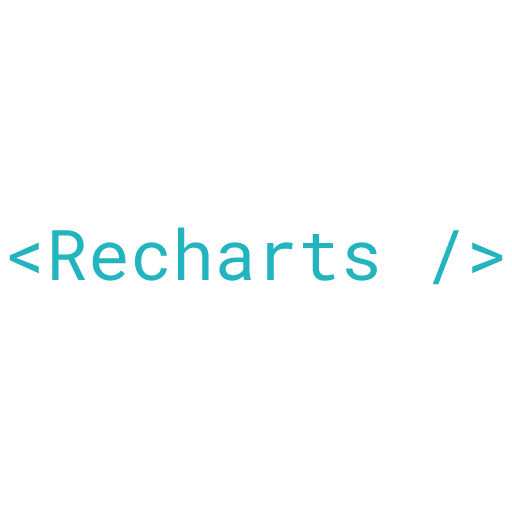
\includegraphics[width=\linewidth]{projet/images/recharts.png}
    \end{minipage}
    \hspace{1cm}
    \begin{minipage}[c]{0.6\textwidth}
        \textbf{Recharts.Js.}\\[0.5em]
    Est Une bibliothèque de graphiques composables construite sur des composants React.Créez rapidement vos graphiques avec des composants React découplés et réutilisables. \cite{ref17}
    \end{minipage}
\end{figure}
\vspace{0.5cm}

\begin{figure}[H]
    \centering
    \begin{minipage}[c]{0.3\textwidth}
        
\includegraphics[width=\linewidth]{projet/images/router-dom.png}
    \end{minipage}
    \hspace{1cm}
    \begin{minipage}[c]{0.6\textwidth}
        \textbf{React Router.}\\[0.5em]
    Est un package npm permettant d'implémenter le routage dynamique dans une application web. Il permet d'afficher des pages et de permettre aux utilisateurs de les parcourir. Il s'agit d'une bibliothèque de routage complète côté client et serveur pour React.  \cite{ref18}
    \end{minipage}
\end{figure}
\vspace{0.5cm}

\begin{figure}[H]
    \centering
    \begin{minipage}[c]{0.3\textwidth}
        
\includegraphics[width=\linewidth]{projet/images/Axios.png}
    \end{minipage}
    \hspace{1cm}
    \begin{minipage}[c]{0.6\textwidth}
        \textbf{Axios.}\\[0.5em]
   Axios, client HTTP basé sur les promesses, fonctionne de manière identique dans node.js et les navigateurs. \cite{ref19}
    \end{minipage}
\end{figure}
\vspace{0.5cm}

\begin{figure}[H]
    \centering
    \begin{minipage}[c]{0.3\textwidth}
        
\includegraphics[width=\linewidth]{projet/images/TanStack Query.png}
    \end{minipage}
    \hspace{1cm}
    \begin{minipage}[c]{0.6\textwidth}
        \textbf{TanStack Query.}\\[0.5em]
    Est une bibliothèque de gestion de l'état du serveur dans les applications React, permettant une gestion efficace des données asynchrones comme les requêtes API. \cite{ref20}
    \end{minipage}
\end{figure}
\vspace{0.5cm}

\begin{figure}[H]
    \centering
    \begin{minipage}[c]{0.3\textwidth}
        
\includegraphics[width=\linewidth]{projet/images/material-ui-.png}
    \end{minipage}
    \hspace{1cm}
    \begin{minipage}[c]{0.6\textwidth}
        \textbf{Material-ui.}\\[0.5em]
    Est une bibliothèque de composants React open-source qui met en
œuvre le design Material de Google. Il est complet et peut être utilisé dans la production à partir du carton. \cite{ref21}
    \end{minipage}
\end{figure}
\vspace{0.5cm}

\begin{figure}[H]
    \centering
    \begin{minipage}[c]{0.3\textwidth}
        
\includegraphics[width=\linewidth]{projet/images/lucide-react.png}
    \end{minipage}
    \hspace{1cm}
    \begin{minipage}[c]{0.6\textwidth}
        \textbf{lucide-react.}\\[0.5em]
    Est  une bibliothèque d'icônes open source proposant plus de 1 000 fichiers vectoriels (SVG) pour l'affichage d'icônes et de symboles dans des projets numériques et non numériques. \cite{ref22}
    \end{minipage}
\end{figure}
\vspace{0.5cm}
\begin{figure}[H]
    \centering
    \begin{minipage}[c]{0.3\textwidth}
        
\includegraphics[width=\linewidth]{projet/images/jwt.png}
    \end{minipage}
    \hspace{1cm}
    \begin{minipage}[c]{0.6\textwidth}
        \textbf{JSON Web Token.}\\[0.5em]
    Est un standard ouvert qui permet une échange sécurisé de tokens entre différentes parties. La sécurité de l’échange
se traduit par la vérification de l’intégrité et de l’authenticité des don-
nées. \cite{ref23}
    \end{minipage}
\end{figure}
\vspace{0.5cm}
\begin{figure}[H]
    \centering
    \begin{minipage}[c]{0.3\textwidth}
        
\includegraphics[width=\linewidth]{projet/images/AOS.png}
    \end{minipage}
    \hspace{1cm}
    \begin{minipage}[c]{0.6\textwidth}
        \textbf{AOS Animate On Scroll.}\\[0.5em]
    Est une bibliothèque open source d'animation par défilement créée par Michał Sajnóg . Elle a été créée pour optimiser les performances en utilisant uniquement du CSS pour les animations et en réservant JavaScript à la gestion de la logique. \cite{ref25}
    \end{minipage}
\end{figure}
\vspace{0.5cm}
\begin{figure}[H]
    \centering
    \begin{minipage}[c]{0.3\textwidth}
        
\includegraphics[width=\linewidth]{projet/images/toast.png}
    \end{minipage}
    \hspace{1cm}
    \begin{minipage}[c]{0.6\textwidth}
        \textbf{React-hot-toast .}\\[0.5em]
    Est une bibliothèque de notifications légère et open source pour React. Comme les autres bibliothèques React Toast, elle est conçue pour imiter les notifications push popularisées par les systèmes d'exploitation natifs, tels qu'iOS et Android, dans les applications web \cite{ref26}
    \end{minipage}
\end{figure}
\section{Architecture adoptée}
\subsection{Architecture logique :}
Avant d’entamer la conception et le développement de tout système informatisé, il est primordial d’élaborer son architecture.  Dans le cadre de notre projet,
nous avons choisi MVC (modèle-Vue-Contrôleur) en tant que patron d’architecture logicielle. Ce dernier permet d’organiser globalement une interface
graphique. En d’autres termes il permet de bien séparer le code de l’interface
graphique de la logique applicative D’ailleurs, c’est un choix populaire pour la
conception d’application web. En général ce modèle permet de distinguer trois
entités qui sont :
\begin{figure}[H]
    \centering
    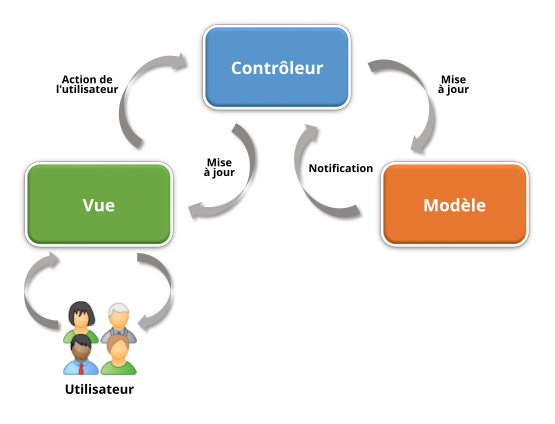
\includegraphics[width=0.6\linewidth]{projet/images/Model-View-Controller.png}
    \caption{L’architecture de Model-View-Controller}
    \label{fig:equipe_scrum}
\end{figure}

\textbf{• Modèle :}\\
contient les données manipulées par le programme. En effet il peut s’agir
d’un ensemble de fonctions (Modèle procédural) ou de classes (Modèle
orienté objet).\\
\textbf{• Vue :}\\
Fait l’interface avec l’utilisateur puisque elle donne plusieurs vues, elle
peut aussi présenter la possibilité à l’utilisateur de changer de vue.\\
\textbf{• Contrôleur :}\\
Un contrôleur contient la logique concernant les actions effectuées par
l’utilisateur.

\subsection{Architecture physique}
Pour assurer de bonnes performances, nous avons choisi une architecture
\textbf{client-serveur}.

Cette architecture est illustrée dans le schéma ci-dessous :

\begin{figure}[H]
    \centering
    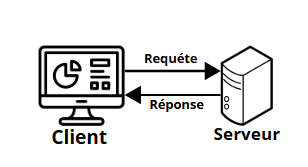
\includegraphics[width=0.6\linewidth]{projet/images/client-serveur.png}
    \caption{L’architecture client-serveur}
    \label{fig:equipe_scrum}
\end{figure}

\begin{itemize}
    \item \textbf{Le client} : que ce soit actif ou bien esclave, il lance la communication avec le serveur en adressant des demandes ou des requêtes.
    \item \textbf{Le serveur} : considéré comme passif ou maître, il répond aux demandes du client.
\end{itemize}

Grâce à cette séparation, chaque partie peut effectuer son travail de manière efficace et améliorer le système.
et plus organisé\\
\section*{Conclution}
Dans ce chapitre, nous avons présenté la planification de notre travail Alors
nous avons dégagé le premier artéfact le backlog de produit qui comporte les tous les liste des fonctionnalités de notre système, Par la suite nous avons dégagé ainsi les différents rôles de l’équipe dans le projet. Enfin nous avons choisi le concept de découpage pour la réalisation des sprints qui vont suivre, Nous allons enchainer à présent avec notre premier sprint dans le
chapitre qui suit.
\chapter{RELEASE 1}
\addcontentsline{toc}{chapter}{Chapitre 3 : RELEASE 1}

\section*{Introduction}
\addcontentsline{toc}{section}{Introduction}
Après avoir exposé en détail les exigences de notre projet à travers un backlog produit, nous entamons dans ce chapitre la première version du projet, qui comprend deux sprints : le sprint 1 et le sprint 2. Chaque sprint couvre l'analyse, la conception et la réalisation.

\section{Organisation du sprint}
Notre release est composée de deux sprints :\\
\textbf{- Sprint 1 :} Configuration initiale et base du projet.\\
\textbf{- Sprint 2 :} Authentification et gestion des utilisateurs.

\section{Sprint 1 : Configuration initiale et base du projet}
\subsection{Objectif du sprint}
L'objectif de ce sprint est de mettre en place l'environnement MERN, la configuration backend et frontend. Les tâches principales sont :
\begin{itemize}
    \item l'initialisation du dépôt Git ;
    \item la création du serveur Express avec une route de test ;
    \item la modélisation de la base de données MongoDB ;
    \item la configuration de React.js et des routes principales.
\end{itemize}

\section{Sprint 2 : Authentification et gestion des utilisateurs}
\subsection{Objectif du sprint}
L'objectif de ce sprint est de mettre en place un système d'authentification (JWT) et une gestion des rôles. Les tâches principales sont :
\begin{itemize}
    \item la création des modèles utilisateurs avec rôles ;
    \item l'implémentation des routes d'authentification et la gestion des sessions avec JWT ;
    \item l'interface React pour l'inscription et la connexion.
\end{itemize}

\subsection{Sprint backlog}
Le deuxième sprint s'étend du 12 février au 21 février. Le tableau suivant représente le backlog de ce sprint.

\renewcommand{\arraystretch}{1.6}
\setlength{\tabcolsep}{5pt}
\begin{longtable}{|c|c|m{7cm}|c|c|}
  \caption{User Stories – Sprint Authentification et gestion des utilisateurs} \\
  \hline
  \textbf{ID} & \textbf{Sprint} & \textbf{User Story} & \textbf{Priorité} & \textbf{Complexité} \\
  \hline
  \endfirsthead
  
  \hline
  \textbf{ID} & \textbf{Sprint} & \textbf{User Story} & \textbf{Priorité} & \textbf{Complexité} \\
  \hline
  \endhead
  
  \hline
  \endfoot
  
  \hline
  \endlastfoot
  
  \multirow{8}{*}{2} & \multirow{8}{*}{\parbox{3cm}{\centering Authentification et\\ gestion des utilisateurs}} 
  & En tant qu'utilisateur, je souhaite créer un compte. & Élevée & Moyenne \\
  \cline{3-5}
  && En tant qu'utilisateur, je souhaite m’authentifier. & Élevée & Moyenne \\
  \cline{3-5}
  && En tant que gestionnaire, je souhaite créer un compte. & Élevée & Moyenne \\
  \cline{3-5}
  && En tant que gestionnaire, je souhaite m’authentifier. & Élevée & Moyenne \\
  \cline{3-5}
  && En tant qu’administrateur, je veux créer un utilisateur pour la gestion des utilisateurs. & Élevée & Moyenne \\
  \cline{3-5}
  && En tant qu’administrateur, je veux modifier un utilisateur pour la gestion des utilisateurs. & Élevée & Moyenne \\
  \cline{3-5}
  && En tant qu’administrateur, je veux supprimer un utilisateur pour la gestion des utilisateurs. & Élevée & Moyenne \\
  \cline{3-5}
  && En tant qu’administrateur, je veux consulter un utilisateur pour la gestion des utilisateurs. & Élevée & Moyenne \\
  \hline
  \end{longtable}

\subsection{Implémentation du sprint 2}
\subsubsection{Spécification des besoins}
Dans cette section, nous identifions les besoins de notre deuxième sprint, à travers :
\begin{itemize}
    \item les diagrammes de cas d'utilisation,
    \item les descriptions textuelles associées,
    \item les diagrammes de séquences système.
\end{itemize}

\textbf{La figure ci-dessous représente le premier diagramme de cas d'utilisation de ce sprint.}

\begin{figure}[H]
    \centering
    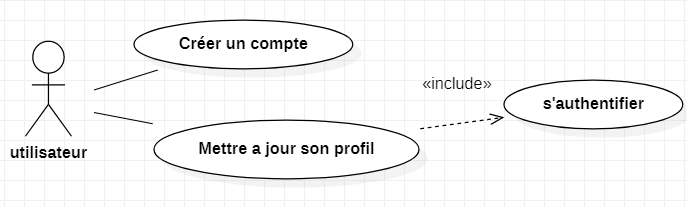
\includegraphics[width=0.6\linewidth]{projet/images/diagramme de sequance/images/utilisateur.png}
    \caption{Diagramme des cas d'utilisation « S'authentifier (Utilisateur) »}
    \label{fig:equipe_scrum}
\end{figure}

Ce diagramme décrit le processus d'authentification de l'utilisateur. Nous détaillons ci-après ce cas d'utilisation sous forme textuelle :

\begin{longtable}{|>{\bfseries}p{4cm}|p{10cm}|}
\hline
Cas d'utilisation & S'inscrire \\
\hline
Acteurs & Utilisateur \\
\hline
Précondition & L'utilisateur demande l'interface d'inscription \\
\hline
Post-condition & Le compte est créé \\
\hline
Scénario principal & 
\begin{enumerate}
  \item Le système affiche la page d'inscription de connexion
  \item L'utilisateur remplit le formulaire et le soumet
  \item Le système vérifie les informations et crée le compte
  \item Le système affiche un message de succès
\end{enumerate} \\
\hline
Scénario alternatif & Le système affiche un message d'erreur si le login ou mot de passe sont incorrects \\
\hline
\caption{Description textuelle du cas d'utilisation pour Créer un compte}
\end{longtable}

\begin{longtable}{|>{\bfseries}p{4cm}|p{10cm}|}
\hline
Cas d'utilisation & S'authentifier (Utilisateur) \\
\hline
Acteurs & Utilisateur \\
\hline
Précondition & L'utilisateur possède un login et un mot de passe \\
\hline
Post-condition & Utilisateur Authentifié \\
\hline
Scénario principal & 
\begin{enumerate}
  \item Le système affiche l'interface qui contient un formulaire de connexion
  \item L'utilisateur saisit son login et son mot de passe
  \item Il confirme en cliquant sur le bouton « se connecter »
  \item Le système affiche l'interface d'accueil propre à l'utilisateur
\end{enumerate} \\
\hline
Scénario alternatif & Le système affiche un message d'erreur si le login ou mot de passe sont incorrects \\
\hline
\caption{Description textuelle du cas d'utilisation « S'authentifier (Utilisateur) »}
\end{longtable}

\textbf{La figure ci-dessous représente le deuxième diagramme de cas d'utilisation de ce sprint.}

\begin{figure}[H]
    \centering
    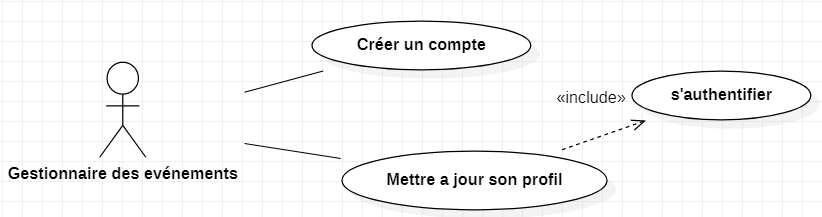
\includegraphics[width=0.6\linewidth]{projet/images/diagramme de sequance/images/gestionnaire.png}
    \caption{Diagramme des cas d'utilisation « S'authentifier (Gestionnaire) »}
    \label{fig:equipe_scrum}
\end{figure}

Ce diagramme décrit le processus d'authentification de gestionnaire. Nous détaillons ci-après ce cas d'utilisation sous forme textuelle :

\begin{longtable}{|>{\bfseries}p{4cm}|p{10cm}|}
\hline
Cas d'utilisation & S'inscrire \\
\hline
Acteurs & Gestionnaire \\
\hline
Précondition & Gestionnaire demande l'interface d'inscription \\
\hline
Post-condition & Le compte est créé \\
\hline
Scénario principal & 
\begin{enumerate}
  \item Le système affiche la page d'inscription de connexion
  \item Gestionnaire remplit le formulaire et le soumet
  \item Le système vérifie les informations et crée le compte
  \item Le système affiche un message de succès
\end{enumerate} \\
\hline
Scénario alternatif & Le système affiche un message d'erreur si le login ou mot de passe sont incorrects \\
\hline
\caption{Description textuelle du cas d'utilisation pour Créer un compte}
\end{longtable}

\begin{longtable}{|>{\bfseries}p{4cm}|p{10cm}|}
\hline
Cas d'utilisation & S'authentifier (gestionnaire) \\
\hline
Acteurs & Gestionnaire \\
\hline
Précondition & L'utilisateur possède un login et un mot de passe \\
\hline
Post-condition & Utilisateur Authentifié \\
\hline
Scénario principal & 
\begin{enumerate}
  \item Le système affiche l'interface qui contient un formulaire de connexion
  \item L'utilisateur saisit son login et son mot de passe
  \item Il confirme en cliquant sur le bouton « se connecter »
  \item Le système affiche l'interface d'accueil propre de gestionnaire
\end{enumerate} \\
\hline
Scénario alternatif & Le système affiche un message d'erreur si le login ou mot de passe sont incorrects \\
\hline
\caption{Description textuelle du cas d'utilisation « S'authentifier (Gestionnaire) »}
\end{longtable}

\textbf{La figure ci-dessous représente le troisième diagramme de cas d'utilisation de ce sprint.}

\begin{figure}[H]
    \centering
    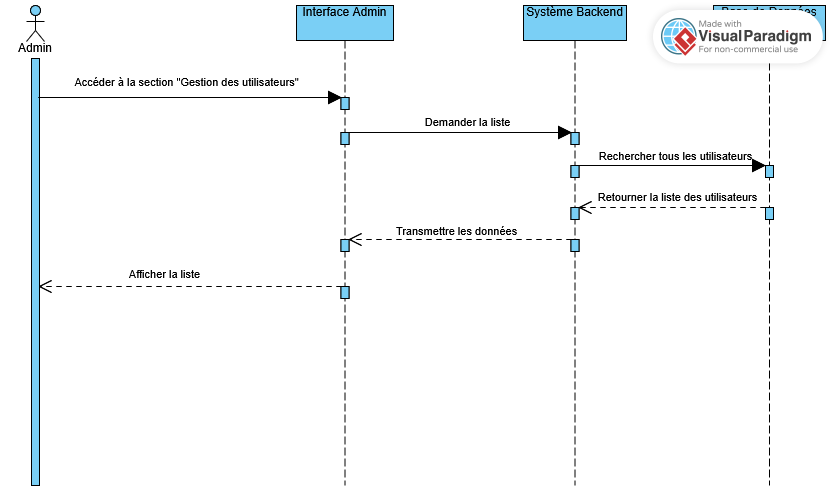
\includegraphics[width=0.6\linewidth]{projet/images/diagramme de sequance/consulter les utilisateurs admin sequnace diagram(1).png}
    \caption{Diagramme des cas d'utilisation « gestion d'utilisation »}
    \label{fig:equipe_scrum}
\end{figure}

Ce diagramme de cas d'utilisation représente le processus de gestion d'utilisateur, qui se manifeste dans l'ajout, la modification, la suppression, la consultation de la liste d'utilisateur. Nous détaillons ci-après ce cas d'utilisation sous forme textuelle :

\begin{longtable}{|>{\bfseries}p{4cm}|p{10cm}|}
\hline
Cas d'utilisation & Créer un utilisateur \\
\hline
Acteurs & Administrateur \\
\hline
Précondition & Authentification préalable \\
\hline
Post-condition & Utilisateur est ajouté \\
\hline
Scénario principal & 
\begin{enumerate}
  \item L'administrateur clique sur le bouton d'ajout d'un utilisateur
  \item Le système affiche le formulaire d'ajout d'un utilisateur
  \item L'administrateur remplit le formulaire avec les informations du l'utilisateur et le soumet
  \item Le système vérifie les informations et ajoute l'utilisateur
  \item Le système affiche un message de succès
\end{enumerate} \\
\hline
Scénario alternatif & 
\begin{enumerate}
  \item L'administrateur soumet le formulaire avec des informations incomplètes ou incorrectes
  \item L'administrateur soumet le formulaire avec les informations d'utilisateur existant
\end{enumerate} \\
\hline
\caption{Description textuelle du cas d'utilisation pour créer un utilisateur}
\end{longtable}

\begin{longtable}{|>{\bfseries}p{4cm}|p{10cm}|}
\hline
Cas d'utilisation & Modifier un utilisateur \\
\hline
Acteurs & Administrateur \\
\hline
Précondition & Authentification préalable \\
\hline
Post-condition & Utilisateur est modifié \\
\hline
Scénario principal & 
\begin{enumerate}
  \item L'administrateur choisit un utilisateur à modifier et clique sur son bouton de modification
  \item Le système affiche le formulaire de modification d'un utilisateur
  \item L'administrateur modifie les informations d'utilisateur et le soumet
  \item Le système vérifie les informations et met à jour les données de l'utilisateur
  \item Le système affiche un message de succès
\end{enumerate} \\
\hline
Scénario alternatif & 
\begin{enumerate}
  \item L'administrateur soumet le formulaire avec des informations incomplètes ou incorrectes
  \item Le système affiche un message d'erreur
\end{enumerate} \\
\hline
\caption{Description textuelle du cas d'utilisation pour modifier un utilisateur}
\end{longtable}

\begin{longtable}{|>{\bfseries}p{4cm}|p{10cm}|}
\hline
Cas d'utilisation & Supprimer un utilisateur \\
\hline
Acteurs & Administrateur \\
\hline
Précondition & Authentification préalable \\
\hline
Post-condition & Utilisateur est supprimé \\
\hline
Scénario principal & 
\begin{enumerate}
  \item L'administrateur choisit un utilisateur et clique sur son bouton de suppression
  \item Le système demande une confirmation de la suppression
  \item L'administrateur confirme la suppression
  \item Le système supprime l'utilisateur
  \item Le système affiche un message de succès
\end{enumerate} \\
\hline
Scénario alternatif & L'administrateur annule la confirmation \\
\hline
\caption{Description textuelle du cas d'utilisation pour supprimer un utilisateur}
\end{longtable}

\begin{longtable}{|>{\bfseries}p{3.5cm}|p{9cm}|}
\hline
Cas d'utilisation & Consulter un utilisateur \\
\hline
Acteurs & Administrateur \\
\hline
Précondition & Authentification préalable \\
\hline
Post-condition & La liste des utilisateurs est affichée \\
\hline
Scénario principal & 
\begin{enumerate}
  \item L'administrateur accède à la page de gestion des utilisateurs
  \item Le système affiche un tableau contenant tous les utilisateurs
\end{enumerate} \\
\hline
Scénario alternatif & Néant \\
\hline
\caption{Description textuelle du cas d'utilisation pour consulter la liste des utilisateurs}
\end{longtable}

\textbf{Les figures ci-après illustrent les diagrammes de séquences systèmes des différents cas d'utilisation de notre 2ème sprint.}

\begin{figure}[H]
    \centering
    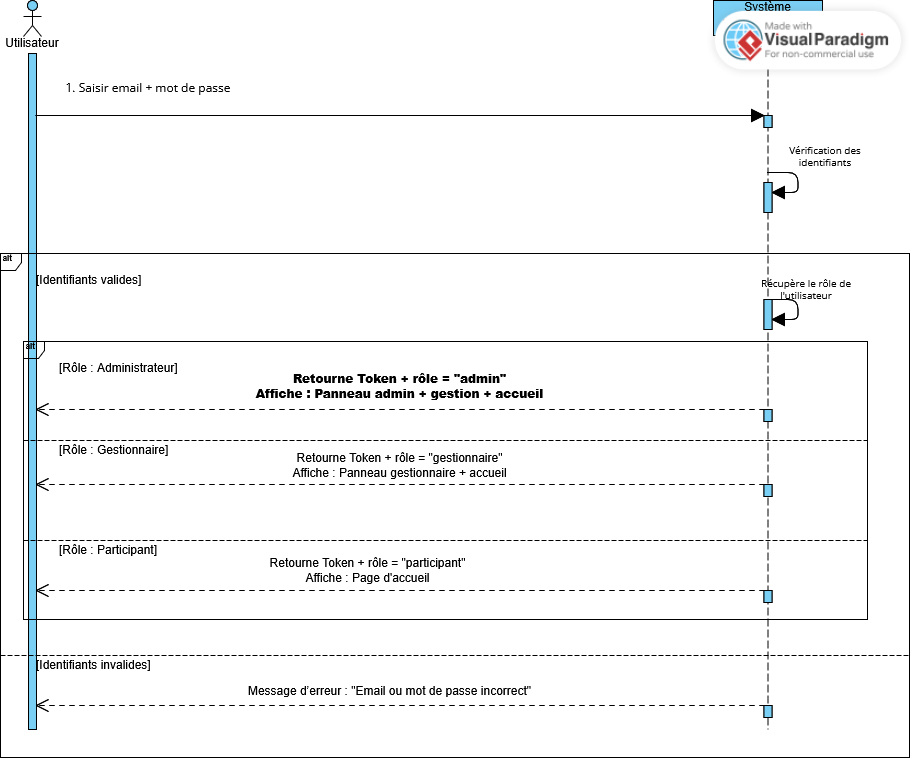
\includegraphics[width=1\linewidth]{projet/images/diagramme de sequance/diagrame de sequance s'athentifier.png}
    \caption{Diagramme de séquence « Authentification »}
    \label{fig:diagramme1}
\end{figure}

\begin{figure}[H]
    \centering
    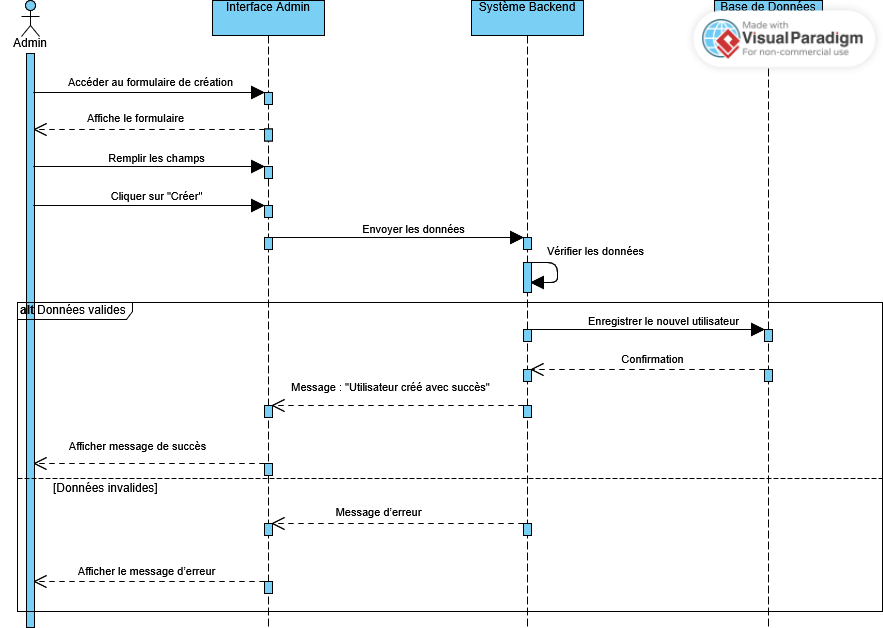
\includegraphics[width=1\linewidth]{projet/images/diagramme de sequance/cree utilisateur admin sequance diagram.png}
    \caption{Diagramme de séquence système Créer un utilisateur}
    \label{fig:diagramme2}
\end{figure}

\begin{figure}[H]
    \centering
    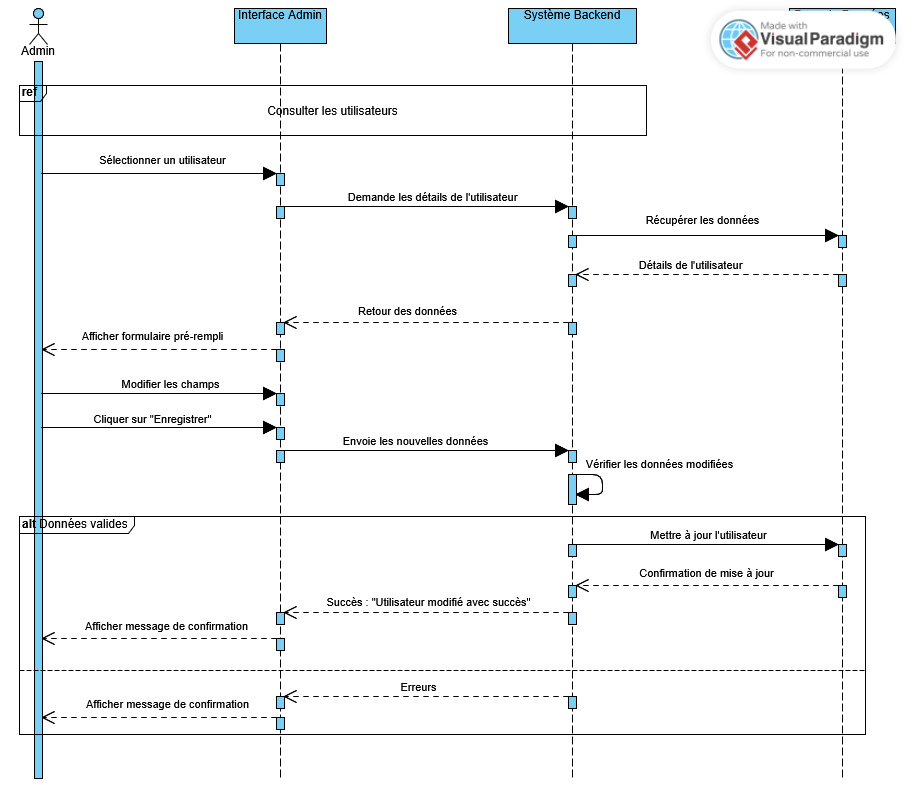
\includegraphics[width=1\linewidth]{projet/images/diagramme de sequance/modifier utlisateur admin sequance diagram.png}
    \caption{Diagramme de séquence système Modifier un utilisateur}
    \label{fig:diagramme3}
\end{figure}

\begin{figure}[H]
    \centering
    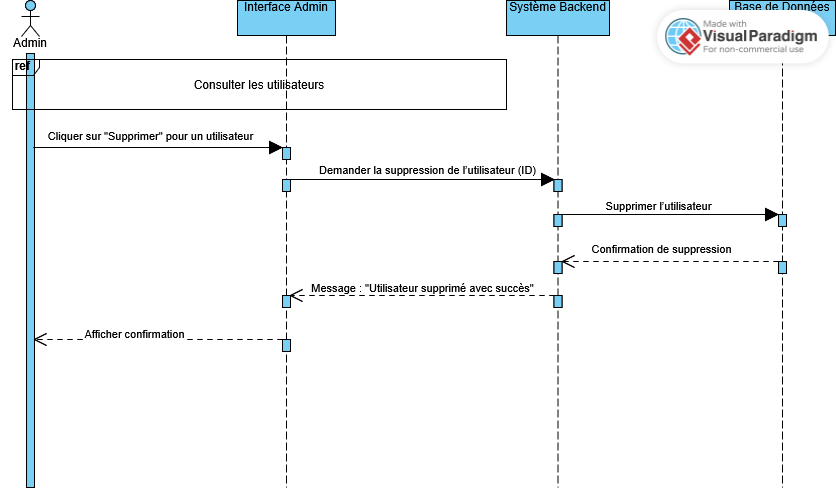
\includegraphics[width=1\linewidth]{projet/images/diagramme de sequance/supprimer utilisateur admin sequance diagram.png}
    \caption{Diagramme de séquence système Supprimer un utilisateur}
    \label{fig:diagramme4}
\end{figure}

\begin{figure}[H]
    \centering
    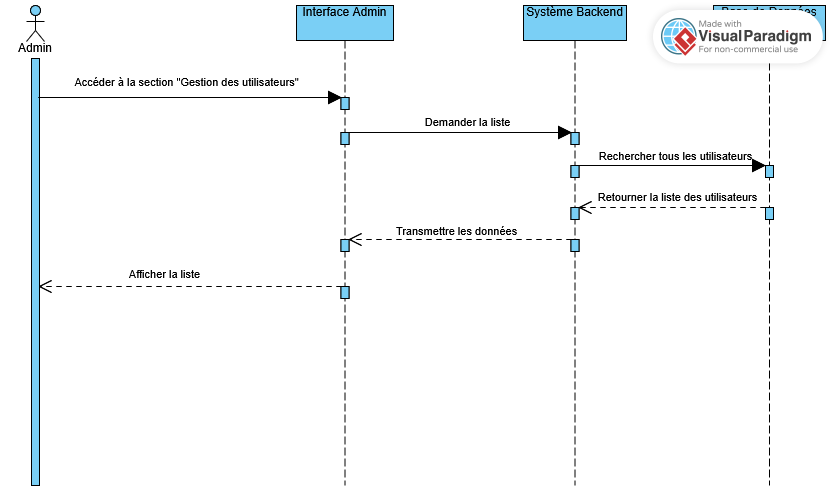
\includegraphics[width=1\linewidth]{projet/images/diagramme de sequance/consulter les utilisateurs admin sequnace diagram(1).png}
    \caption{Diagramme de séquence système Consulter un utilisateur}
    \label{fig:diagramme5}
\end{figure}

\textbf{Diagramme de classe (à compléter)}

\subsubsection{Réalisation}
Cette interface représente le formulaire d'inscription dédié à l'utilisateur et gestionnaire, comprenant les champs nom mail mot de passe.

\begin{figure}[H]
    \centering
    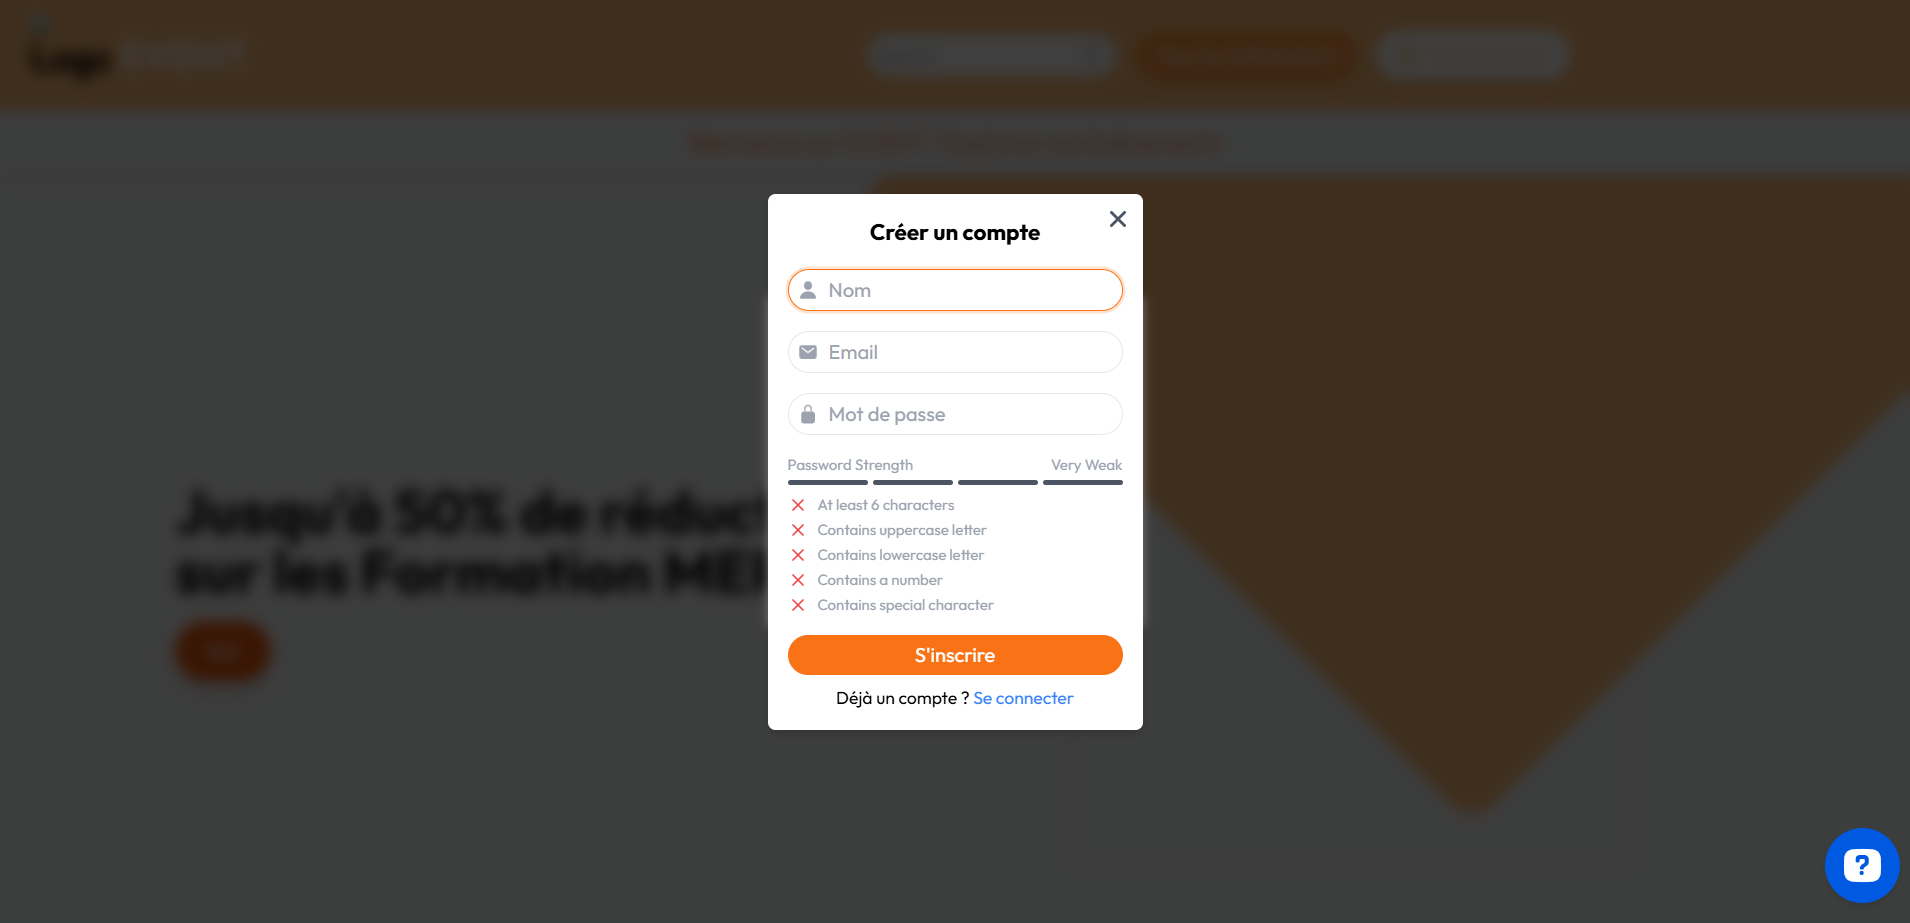
\includegraphics[width=1\linewidth]{projet/images/diagramme de sequance/images/registration.png}
    \caption{Interface graphique de creation compte}
    \label{fig:interface1}
\end{figure}

\begin{figure}[H]
    \centering
    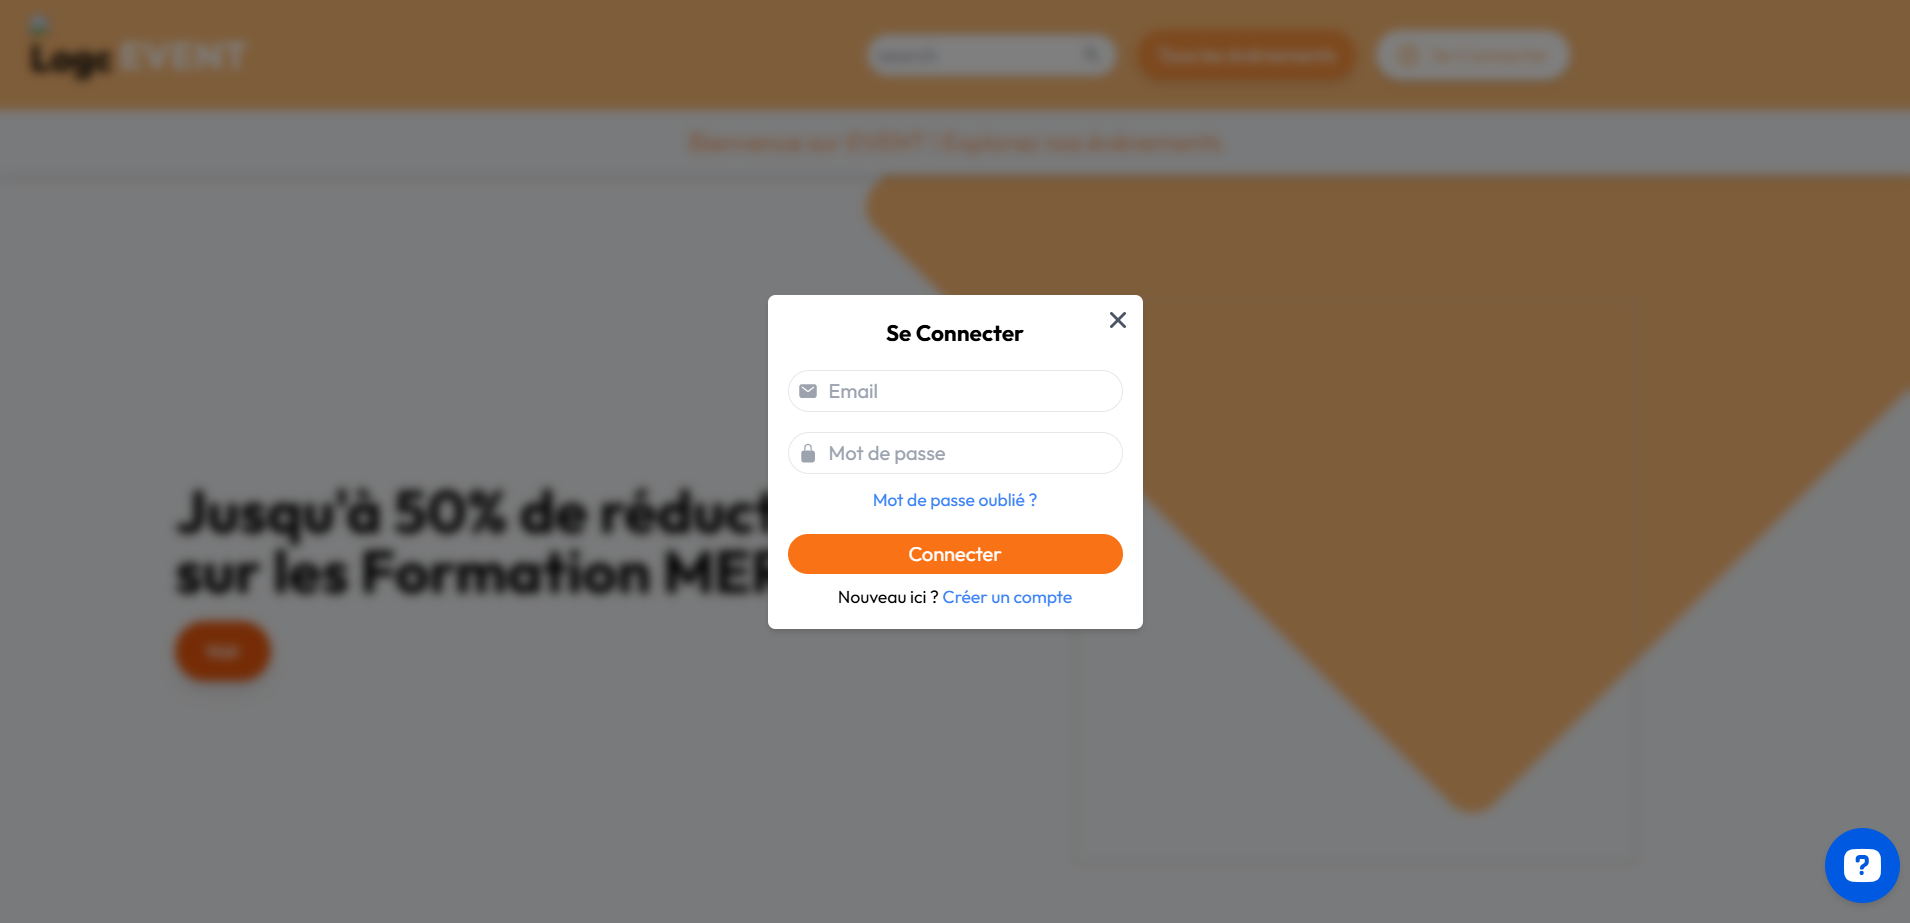
\includegraphics[width=1\linewidth]{projet/images/diagramme de sequance/images/login.png}
    \caption{Interface graphique d'authentification}
    \label{fig:interface2}
\end{figure}

Cette interface représente la page d'accueil de l'administrateur. Elle s'affiche une fois la gestion des utilisateurs.

\begin{figure}[H]
    \centering
    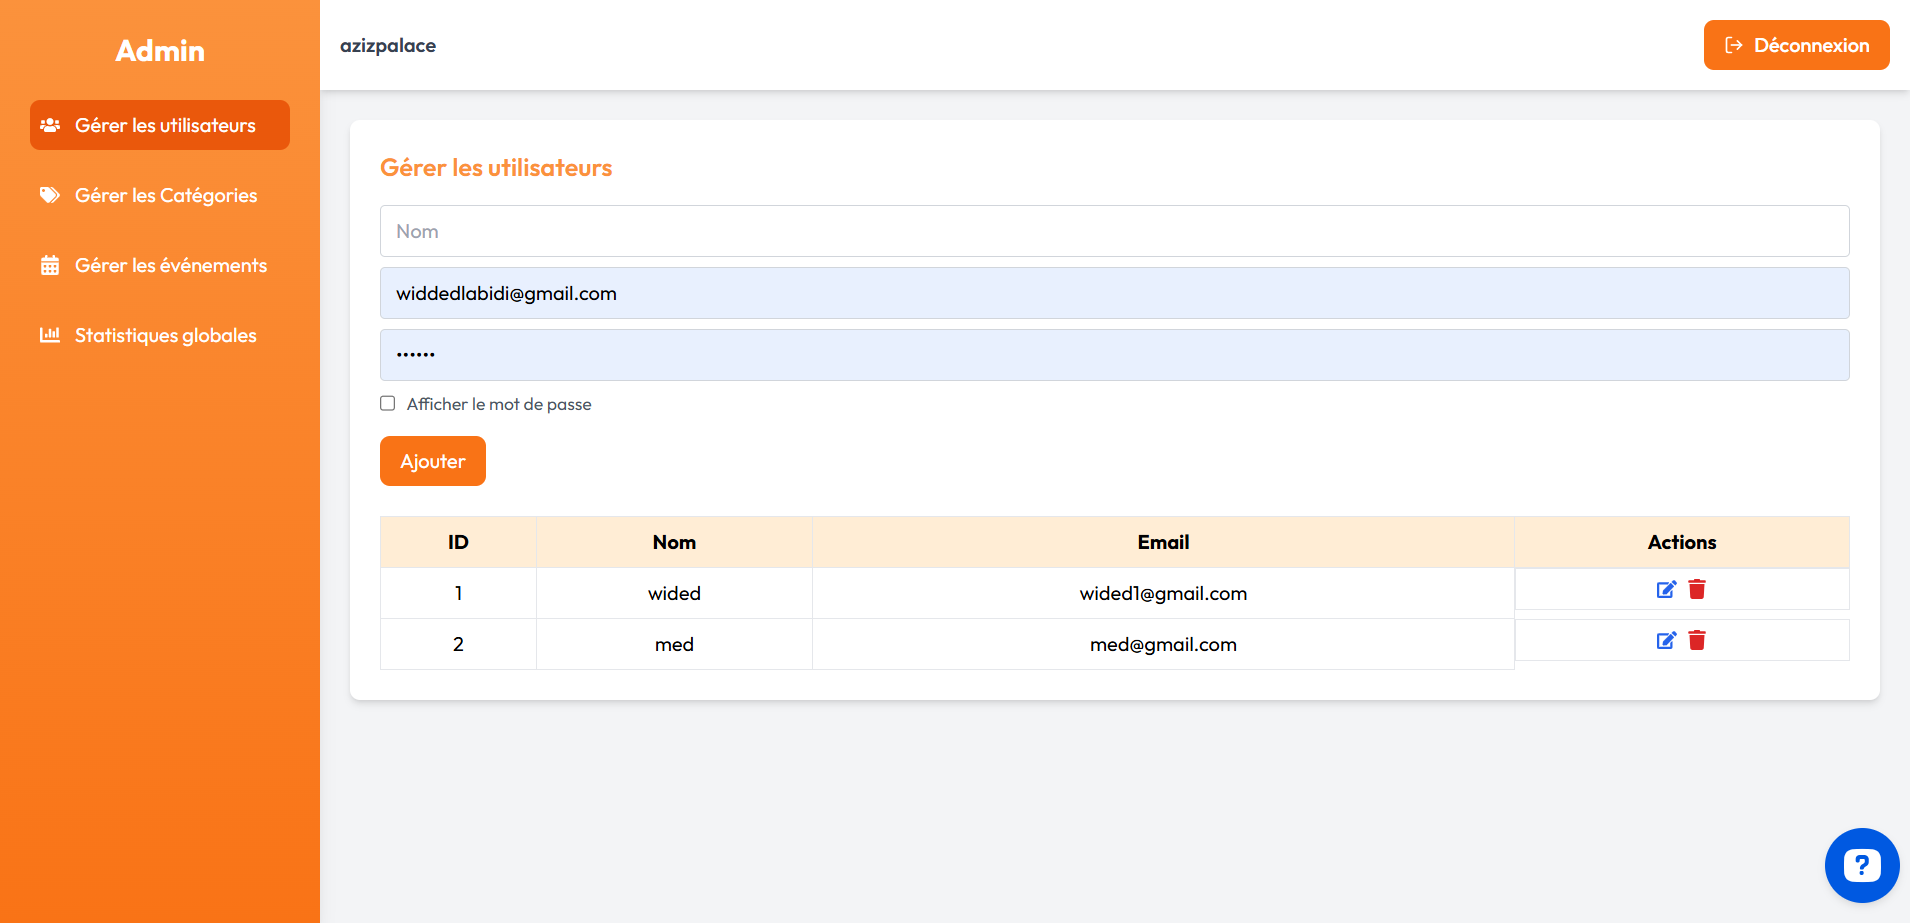
\includegraphics[width=1\linewidth]{projet/images/diagramme de sequance/images/gestion d'utilisateur.png}
    \caption{Interface graphique de gérer les utilisateurs}
    \label{fig:interface3}
\end{figure}
\chapter{RELEASE 2}
\addcontentsline{toc}{chapter}{Chapitre 4 : RELEASE 2}

 

 \addcontentsline{toc}{section}{Introduction} % Ajoute "Introduction" dans la table des matières

\section*{Introduction}

\chapter{Inscription et interaction utilisateur   }
\addcontentsline{toc}{chapter}{Chapitre 5 : Inscription et interaction utilisateur }

\section*{Introduction}
\addcontentsline{toc}{section}{Introduction}
Dans ce chapitre, nous allons étudier en profondeur la quatrième sprint de notre projet. 
\section{Organisation du sprint}
Notre chapitre est composée par :\\
\textbf{Sprint 4 :} Inscription et interaction utilisateur
\section{Sprint 4 : Inscription et interaction utilisateur}
\subsection{Objectif du sprint}\\
L'objectif de ce sprint est l'inscription aux événements et feedback utilisateur, et après tout ça le participant pourra consulter les événements.

\subsection{Sprint backlog}
Le 4éme sprint s’étend du  05 mars au 14 mars. Le tableau suivant représente le backlog de ce sprint:
\begin{table}[h!]
\renewcommand{\arraystretch}{1.6}
\setlength{\tabcolsep}{5pt}
\centering
\begin{tabular}{|c|c|m{7cm}|c|c|}
\hline
\textbf{ID} & \textbf{Sprint} & \textbf{User Story} & \textbf{Priorité} & \textbf{Complexité} \\
\hline
\multirow{5}{*}{4} & \multirow{5}{*}{\parbox{3cm}{\centering Inscription et interaction utilisateur}}
& En tant que Participant. je veux consulter les évenement & Élevée & Faible \\
\cline{3-5}
&& En tant que Participant. je veux  Inscrire a un évenement. & Moyenne & Faible \\
\cline{3-5}
&& En tant que Participant. je veux  Annuler l'inscription "en attente" . & Moyenne & Faible \\
\cline{3-5}
&&En tant que Participant. je veux  Envoyer des messages pour demande d'information & Moyenne & Faible\\
\cline{3-5}
&& En tant que Participant , je veux faire des commentaires & Moyenne & Trés  faible \\
\hline
\end{tabular}
\end{table}
\subsection{Implémentation du sprint 4}
\subsubsection{Spécification des besoins}
Dans cette section, nous identifions les besoins de notre  sprint, à travers :
\begin{itemize}
    \item les diagrammes de cas d’utilisation,
    \item les descriptions textuelles associées,
    \item les diagrammes de séquences système.
\end{itemize}

\textbf {La figure ci-dessous représente le diagramme de cas d’utilisation de ce sprint par rapport aux participants.}
\begin{figure}[H]
    \centering
    \includegraphics[width=0.6\linewidth]{projet/images/sprint4/partisipant1.png}
    \caption{Diagramme des cas d’utilisation d'inscription et interaction utilisateur }
    \label{fig:Adminee }
\end{figure}
\clearpage
Ce diagramme décrit le processus d'inscription et interaction utilisateur pour le Participant. Nous détaillons ci-après ce cas d’utilisation sous forme textuelle :

\begin{longtable}{|>{\bfseries}p{4cm}|p{10cm}|}
\hline
Cas d’utilisation & Consutler un événement \\
\hline
Acteur & Participant \\
\hline
Précondition & Le Participant est authentifié \\
\hline
Post-condition & Les événements sont affichés \\
\hline
Scénario principal & 
\begin{enumerate}
  \item le Participant accède à la page d’accueil ou de recherche.
  \item  Le système affiche la liste des événements disponibles
\end{enumerate} 
\hline
Scénario alternatif &  Aucun événement n’est disponible : un message “Aucun événement disponible” est affiché.
\hline
\caption{Description textuelle du cas d’utilisation pour consutler  un événement}
\end{longtable}


\begin{longtable}{|>{\bfseries}p{4cm}|p{10cm}|}
\hline
Cas d’utilisation & S'inscrire à un événement \\
\hline
Acteur & Participant \\
\hline
Précondition & Être connecté et consulter un événement\\
\hline
Post-condition & Le participant est inscrit à l’événement \\
\hline
Scénario principal & 
\begin{enumerate}
  \item le Participant choisit un événement.
  \item   Il clique sur "S'inscrire maintenant".
  \item Le système affiche les détails du paiement 
  \item le participant  saisit les informations nécessaires et clique sur  "Procéder au paiement".
\item Le système affiche une nouvelle page contenant :(Le prix,RIB )
\item Le participant clique sur button "Valider le paiement".
\item Le système enregistre l’intention de paiement et affiche un message de confirmation .

\end{enumerate} 
\hline
Scénario alternatif &  Le participant ferme la page avant de valider le paiement

\hline
\caption{Description textuelle du cas d’utilisation pour inscrire à un événement}
\end{longtable}
\clearpage
\begin{longtable}{|>{\bfseries}p{4cm}|p{10cm}|}
\hline
Cas d’utilisation & Annuler l'inscription "en attente" \\
\hline
Acteur & Participant \\
\hline
Précondition &
\begin{enumerate}
  \item Être connecté .
  \item L'inscription a le statut "en attente"
  \end{enumerate} 
\hline
Post-condition & 
\begin{enumerate}
    \item Si l'inscription est encore en attente, elle est annulée avec succès (supprimée ou marquée comme "annulée").
    \item Si l'inscription est déjà validée, on ne peut pas faire l'annulation
\end{enumerate}
\hline
Scénario principal & 
\begin{enumerate}
  \item le Participant Accède à "Mon profil".
  \item Le système affiche les inscription en attente 
  \item le participant sélectionne une inscription avec le statut “en attente” et Il clique sur “Annuler”
\item Le système affiche un message "Êtes-vous sûr de vouloir annuler cette inscription ?" 
\item  Le Participant clique sur “OK”
\item  Le système affiche le message : “Inscription supprimée avec succès”

\end{enumerate} 
\hline
Scénario alternatif & Le Participant clique sur “Non” dans la boîte de confirmation : aucune action n’est effectuée.
\hline
\caption{Description textuelle du cas d’utilisation pour annuler l’inscription "en attente"}
\end{longtable}

\begin{longtable}{|>{\bfseries}p{4cm}|p{10cm}|}
\hline
Cas d’utilisation & Envoyer des messages pour demande d'information \\
\hline
Acteur & Participant \\
\hline
Précondition & Le participant est connecté au site.\\
\hline
Post-condition & La demande est envoyée à l'admin\\
\hline
Scénario principal & 
\begin{enumerate}
  \item Le participant accéde à la page de contact.
  \item Le participant  saisit son adresse e-mail dans le champ prévu.et rédige son message et clique sur "Envoyer"
  \item Le système affiche un message de confirmation 
  (« Message envoyé avec succès »).
  \item Le message est envoyé à l’administrateur.
\end{enumerate} 
\hline
Scénario alternatif & Le système affiche un message d’erreur : « Veuillez remplir tous les champs correctement. »
\hline
\caption{Description textuelle du cas d’utilisation pour Envoyer des messages pour demande d’information .}
\end{longtable}


\begin{longtable}{|>{\bfseries}p{4cm}|p{10cm}|}
\hline
Cas d’utilisation & Faire un commentaire \\
\hline
Acteur & Participant \\
\hline
Précondition & 
\begin{enumerate}
  \item Le participant est connecté au site.
  \item L’événement n’est pas encore terminé.
\end{enumerate} 
\hline
Post-condition & Le commentaire est visible par les autres \\
\hline
Scénario principal & 
\begin{enumerate}
  \item Le participant accède à la page d’un événement.
  \item Le système vérifie que l’événement est encore actif.
  \item Dans la section "Laissez un commentaire", il écrit un message et clique sur le bouton Publier.
  \item Le système enregistre et affiche le commentaire. 
  
\end{enumerate} \\
\hline

Scénario alternatif & 
\begin{enumerate}
  \item Si le participant non connecté tente d'accéder à la section commentaire,
  \item Le champ de saisie et le bouton Publier sont désactivés ou masqués.
\end{enumerate} 
\hline
\caption{Description textuelle du cas d’utilisation pour Faire un commentaire.}
\end{longtable}



\chapter*{Conclusion Générale}
%ajouter le titre introduction générale dans la table des matières
\addcontentsline{toc}{chapter}{Conclusion Générale}
%définir l'entête de ce chapitre 
\markboth{Conclusion Générale}{}


\addcontentsline{toc}{chapter}{Références} % Ajout dans la table des matières

\begin{thebibliography}{99}

\bibitem{ref1}
 \url{https://www.lucidchart.com/pages/tutorial/uml}  


\bibitem{ref2}
  \url{https://slack.com/intl/fr-fr/blog/collaboration/methode-agile} 
  \bibitem{ref3}
  \url{https://asana.com/fr/resources/what-is-scrum}
.  \bibitem{ref4}
  \url{lhttps://bility.fr/definition-visual-studio-code/}
  \bibitem{ref5}
\url{https://www.postman.com/product/what-is-postman/}
 \bibitem{ref6}
\url{https://nodejs.org/en/}
\bibitem{ref7}
\url{https://www.lemagit.fr/definition/GitHub}
\bibitem{ref8}
\url{https://scosi.univ-littoral.fr/assistance/catalogue-de-services/overleaf/#:~:text=Overleaf%20est%20un%20%C3%A9diteur%20LaTeX,documents%20scientifiques%20de%20hautes%20qualit%C3%A9s.}
\bibitem{ref9}
\url{https://developer.mozilla.org/fr/docs/Web/HTML}
\bibitem{ref10}
\url{https://developer.mozilla.org/en-US/docs/Web/CSS}
\bibitem{ref11}
\url{https://developer.mozilla.org/en-US/docs/Web/JavaScript}
\bibitem{ref12}
\url{https://www.techno-science.net/glossaire-definition/LaTeX.html}
\bibitem{ref13}
\url{https://fr.wikipedia.org/wiki/Tailwind_CSS}
\bibitem{ref14}
\url{https://kinsta.com/fr/base-de-connaissances/qu-est-express-js/}
\bibitem{ref15}
\url{https://www.mongodb.com/fr-fr/company/what-is-mongodb}
\bibitem{ref16}
\url{https://kinsta.com/fr/base-de-connaissances/qu-est-react-js/}
\bibitem{ref17}
\url{https://recharts.org/en-US}
\bibitem{ref18}
\url{https://www.geeksforgeeks.org/what-is-react-router-dom/}
\bibitem{ref19}
\url{https://axios-http.com/docs/intro}
\bibitem{ref20}
\url{https://medium.com/@ignatovich.dm/tanstack-query-a-powerful-tool-for-data-management-in-react-0c5ae6ef037c}
\bibitem{ref21}
\url{https://mui.com/}
\bibitem{ref22}
\url{https://lucide.dev/guide/}
\bibitem{ref23}
\url{https://jwt.io/introduction}
\bibitem{ref24}
\url{https://vite.dev/guide/}
\bibitem{ref25}
\url{https://shanelonergan.github.io/animate-on-scroll-react/}
\bibitem{ref26}
\url{https://refine.dev/blog/react-hot-toast/#what-is-react-hot-toast}
\bibitem{ref27}
\url{https://www.canva.com/fr_fr/about/}


\end{thebibliography}

\end{document}
